\chapter{Systematic uncertainty}
\label{ch:sys-unc}

\par Once signal regions are determined, one can use the data observations and its systematic uncertainties in signal regions to do statistical analysis. Data observation is easy to obtain with signal region determined, while its systematic uncertainties are not trivial to calculate. In this analysis, both experimental and theoretical uncertainties are considered.

\section{Experimental systematics}

\par Experimental uncertainty is the systematic uncertainty that comes from reconstruction of physics objects. It is a reflection of uncertainty related to detectors or reconstruction algorithms. Multiple physical objects, like muon, electron, jets, \met, etc., are used in this analysis. Therefore, the systematic uncertainties of the reconstruction of these variables needed to be considered carefully when interpreting the analysis result. A summary of these experimental uncertainties can be viewed in Table~\ref{tab:c8:expsyst1}, Table~\ref{tab:c8:expsyst2} and Table~\ref{tab:c8:expsyst3}.

\begin{table}[h]
    \scriptsize
    \begin{center}
        \begin{tabular}{ll}
            \hline
            \hline
            Systematic uncertainty & Short description \\
            \hline
            \multicolumn{2}{c}{\textbf{Event}} \\
            \hline
            Luminosity & Uncertainty on the total integrated luminosity \\
            \hline
            \multicolumn{2}{c}{\textbf{Electrons}} \\
            \hline
            EL\_EFF\_Trigger\_TOTAL\_1NPCOR\_PLUS\_UNCOR & Trigger efficiency uncertainty \\
            EL\_EFF\_Reco\_TOTAL\_1NPCOR\_PLUS\_UNCOR & Reconstruction efficiency uncertainty \\
            EL\_EFF\_ID\_TOTAL\_1NPCOR\_PLUS\_UNCOR & ID efficiency uncertainty \\
            EL\_EFF\_Iso\_TOTAL\_1NPCOR\_PLUS\_UNCOR & Isolation efficiency uncertainty \\
            EG\_SCALE\_ALL & Energy scale uncertainty \\
            EG\_RESOLUTION\_ALL & Energy resolution uncertainty \\
            \hline
            \multicolumn{2}{c}{\textbf{Muons}} \\
            \hline
            mu20\_iloose\_L1MU15\_OR\_HLT\_mu40\_MUON\_EFF\_Trig & Trigger efficiency uncertainties \\ 
			mu24\_ivarmed\_OR\_HLT\_mu40\_MU\_EFF\_TrigStat & None \\ 
			mu24\_ivarmed\_OR\_HLT\_mu50\_MU\_EFF\_TrigStat & None \\ 
			mu26\_ivarmed\_OR\_HLT\_mu50\_MU\_EFF\_TrigStat & None \\ 
            MUON\_EFF\_RECO\_STAT & Reconstruction uncertainty for \pt $>15GeV$ \\
            MUON\_EFF\_RECO\_SYS & None \\ 
			MUON\_EFF\_RECO\_STAT\_LOWPT & \speciallcell{Reconstruction and \\ID efficiency uncertainty for \pt $<15GeV$} \\ 
			MUON\_EFF\_RECO\_SYS\_LOWPT & None \\ 
			MUON\_ISO\_STAT & Isolation efficiency uncertainty \\ 
			MUON\_ISO\_SYS & None \\ 
			MUON\_TTVA\_STAT & Track-to-vertex association efficiency uncertainty \\ 
			MUON\_TTVA\_SYS & None \\ 
            MUONS\_SCALE & Energy scale uncertainty \\
            MUONS\_SAGITTA\_RHO & Variations in the scale of the momentum \\
            MUONS\_SAGITTA\_RESBIAS & Variations in the scale of the momentum \\
            MUONS\_ID & Energy resolution uncertainty from inner detector \\
            MUONS\_MS & Energy resolution uncertainty from muon system \\
            \hline
            \multicolumn{2}{c}{\textbf{\met related}} \\
            \hline
            METTrigStat & Trigger efficiency uncertainty \\
            METTrigSyst & None \\
            MET\_SoftTrk\_ResoPerp & \speciallcell{Track-based soft term related to \\transversal resolution uncertainty} \\ 
			MET\_SoftTrk\_ResoPara & \speciallcell{Track-based soft term related to \\longitudinal resolution uncertainty} \\
			MET\_SoftTrk\_Scale & \speciallcell{Track-based soft term related to \\longitudinal scale uncertainty} \\
			MET\_JetTrk\_Scale  & \speciallcell{Track \met scale uncertainty \\due to tracks in jets} \\
            PRW\_DATASF & \speciallcell{Uncertainty on data scale factor used \\for the computation of pileup reweighting} \\
            \hline
            \hline
		\end{tabular}
	\end{center}
	\caption{A summary of the experimental systematic uncertainties.}
	\label{tab:c8:expsyst1}
\end{table}

\begin{table}[h]
    \scriptsize
    \begin{center}
        \begin{tabular}{ll}
            \hline
            \hline
            Systematic uncertainty & Short description \\
            \hline
            \multicolumn{2}{c}{\textbf{Small-radius jets}} \\
            \hline
            JET\_EtaIntercalibration\_Modelling & $\eta$-intercalibration: MC generator modelling uncertainty \\
            JET\_EtaIntercalibration\_TotalStat & $\eta$-intercalibration: statistical uncertainty \\
            JET\_EtaIntercalibration\_NonClosure\_highE & \speciallcell{$\eta$-intercalibration: non-closure uncertainty \\of jet response, high energy component} \\
            JET\_EtaIntercalibration\_NonClosure\_negEta & \speciallcell{$\eta$-intercalibration: non-closure uncertainty \\of jet response, negative $\eta$ component} \\
            JET\_EtaIntercalibration\_NonClosure\_posEta & \speciallcell{$\eta$-intercalibration: non-closure uncertainty \\of jet response, positive $\eta$ component} \\
            JET\_Pileup\_OffsetMu & Pileup: Offset, term for number of interactions per crossing $\mu$ \\
            JET\_Pileup\_OffsetNPV & Pileup: Offset, term for number of primary vertices \\
            JET\_Pileup\_PtTerm & Pileup: Offset, \pt term \\
            JET\_Pileup\_RhoTopology & Pileup: Offset, $\rho$ topology uncertainty on jet areas \\
            JET\_Flavor\_Composition & Flavor composition uncertainty \\
            JET\_Flavor\_Response &  Flavor response uncertainty (dominated by gluon response) \\
            JET\_PunchThrough\_MC16 & Punch-through correction uncertainty \\
            JET\_EffectiveNP\_Statistical & \speciallcell{Statistical components of effective jet energy scale uncertainties, \\split into 6 components} \\
            JET\_EffectiveNP\_Modelling & \speciallcell{Modelling components of effective jet energy scale uncertainties, \\split into 4 components} \\
            JET\_EffectiveNP\_Detector & \speciallcell{Detector components of effective jet energy scale uncertainties, \\split into 2 components} \\
            JET\_EffectiveNP\_Mixed & \speciallcell{Effective jet energy scale uncertainties coming from various sources, \\split into 3 components} \\
            JET\_SingleParticle\_HighPt & Uncertainty related to high \pt jets \\
            JET\_RelativeNonClosure\_MC16 & Closure of the calibration, relative to MC12a \\
            JET\_BJES\_Response & Jet energy scale uncertainty for $b$-jets \\
            JET\_JER\_DataVsMC\_MC16 & \speciallcell{Nuisance parameter covering when jet energy resolution \\in data smaller than resolution in MC} \\
            JET\_JER\_EffectiveNP & Effective jet energy resolution uncertainty; split into 6 components \\
            FT\_EFF\_EIGEN\_B & $b$-tagging efficiency uncertainties ("BTAG\_MEDIUM) \\
            FT\_EFF\_EIGEN\_C & None \\
            FT\_EFF\_EIGEN\_L & None \\
            FT\_EFF\_EIGEN\_extrapolation & $b$-tagging efficiency uncertainty on the extrapolation on high \pt-jets \\
            FT\_EFF\_EIGEN\_extrapolation\_from\_charm & $b$-tagging efficiency uncertainty on $\tau$-jets \\
            \hline
            \hline
        \end{tabular}
	\end{center}
	\caption{A summary of the experimental systematic uncertainties.}
	\label{tab:c8:expsyst2}
\end{table}

\begin{table}[h]
    \scriptsize
    \begin{center}
        \begin{tabular}{ll}
            \hline
            \hline
            Systematic uncertainty & Short description \\
            \hline
            \multicolumn{2}{c}{\textbf{Large-radius jets}} \\
            \hline
            JET\_EtaIntercalibration\_Modelling & $\eta$-intercalibration: MC generator modelling and method uncertainty \\
            JET\_EtaIntercalibration\_R10\_TotalStat & $\eta$-intercalibration: statistical uncertainty \\
            JET\_Flavor\_Composition & Flavor composition uncertainty \\
            JET\_Flavor\_Response & Flavor response uncertainty (dominated by gluon response) \\
            JET\_EffectiveNP\_R10\_Statistical & \speciallcell{Statistical components of effective jet energy scale uncertainties, \\split into 6 components} \\
            JET\_EffectiveNP\_R10\_Modelling & \speciallcell{Modelling components of effective jet energy scale uncertainties, \\split into 4 components} \\
            JET\_EffectiveNP\_R10\_Detector & \speciallcell{Detector components of effective jet energy scale uncertainties, \\split into 2 components} \\
            JET\_EffectiveNP\_R10\_Mixed & \speciallcell{Effective jet energy scale uncertainties coming from various sources, \\split into 3 components} \\
            JET\_SingleParticle\_HighPt & Uncertainty related to high \pt jets (for R=0.4) \\
            JET\_CombMass\_Baseline	& \speciallcell{Baseline uncertainty of the jet mass scale \\accounting for data-MC differences} \\
            JET\_CombMass\_Modelline & \speciallcell{Modelling uncertainty of the jet mass scale \\accounting for different MC generators} \\
            JET\_CombMass\_Tracking	& \speciallcell{Uncertainty of the jet mass scale accounting \\for tracking variations; 3 variations in total} \\
            \hline
            \multicolumn{2}{c}{\textbf{Variable-radius track jets}} \\
            \hline
            FT\_EFF\_EIGEN\_B & $b$-tagging efficiency uncertainties \\
            FT\_EFF\_EIGEN\_C & None \\
            FT\_EFF\_EIGEN\_L & None \\
            FT\_EFF\_EIGEN\_extrapolation & $b$-tagging efficiency uncertainty on the extrapolation on high \pt-jets \\
            FT\_EFF\_EIGEN\_extrapolation\_from\_charm & $b$-tagging efficiency uncertainty on $\tau$-jets \\
            \hline
            \hline
        \end{tabular}
	\end{center}
	\caption{A summary of the experimental systematic uncertainties.}
	\label{tab:c8:expsyst3}
\end{table}

\section{Theoretical systematics}

\par Theoretical uncertainty is the systematic uncertainty that comes from Monte-Carlo simulation of background and signal processes. In this analysis, both the signal and background yields come from monte carlo simulation samples rather than data driven estimation from control regions. Therefore, a careful estimation on theoretical uncertainties is needed on all related simulation processes.

\par The sources of theoretical uncertainty are listed below:

\begin{itemize}
    \item \textbf{Missing higher orders in the calculation of the inclusive matrix elements}: For all processes the calculation of the cross-section relies on a perturbative expansion of the scattering matrix, which is truncated at a certain order. The effect of the missing higher orders is estimated by varying the renormalisation and factorisation scales ($\mu_R$ and $\mu_F$) independently by a factor of 2, excluding the $(\mu_R,\mu_F)=(\frac{1}{2},2),(2,\frac{1}{2})\times \mu_{\text{central}}$ variations, which may lead to large logarithms. 
    \item \textbf{Uncertainties from the choice of PDFs and $\alpha_s$}: This kind of uncertainty arises from uncertainties in the experimental measurements that are used to determine the PDF sets used in each calculation, uncertainties from the choice of the functional form used in the PDF fits, and uncertainties associated to the experimental determination of $\alpha_s$. These are estimated using the PDF4LHC prescription\cite{Butterworth_2016}.
    \item \textbf{Merging scale uncertainties}: For samples generated by merging matrix elements (ME) corresponding to different multiplicities, e.g. $V+jets$, an uncertainty related to the choice of the merging scale, i.e. the scale that separates soft from hard jets, is evaluated by varying the merging scale by a factor of 2 up and down.
    \item \textbf{Resummation scale uncertainties}: For \textsc{Sherpa}\cite{Gleisberg_2009} samples an additional uncertainty related to the energy cut-off for the integration of MC counterterms in the parton shower (PS).
    \item \textbf{Matching uncertainties}: For samples generated using a NLO matrix element and matched to a parton shower, a comparison between a \textsc{Powheg} and a \textsc{MG5aMC} sample can probe uncertainties related to the ME/PS matching procedure.
    \item \textbf{Parton shower/Hadronisation uncertainties}: Uncertainties related to algorithmic or parametric differences in the modelling of the PS and hadronisation can be assessed by comparing samples generated with different showering/hadronisation (SHG) generators, typically \textsc{Pythia~8} with \textsc{Herwig~7}.  
    \item \textbf{Eigentune uncertainties}: This kind of uncertainties are related to uncertainties in the choice of the free parameters that are used in the SHG programmes, derived so as to encompass the data used in the ATLAS tuning program\cite{ATL-PHYS-PUB-2014-021}.
    \item \textbf{Other implementation-specific uncertainties}: The variation of the $h_{\text{damp}}$ scale in the \text{Powheg} samples, etc..
\end{itemize}

\par The sources mentioned above are considered and grouped into Monte-carlo template, which is used as an input of the likelihood fit. There are four types of uncertainties considered in the statistical interpretation:

\begin{enumerate}
    \item \textbf{Inclusive cross-section uncertainties}: Inclusive cross-section uncertainties are implemented in the fit using Gaussian priors that affect the normalisation of a given samples in all regions in a correlated manner (\texttt{OverallSys} in the \textsc{HistFactory} terminology \cite{Cranmer:1456844}). These uncertainties are applied only on the samples whose normalisation is not freely floating in the fit.
    \item \textbf{Shape uncertainties}: Shape uncertainties are uncertainties on the shape of the fitted discriminant ($m(b\bar{b})$). These uncertainties are estimated by comparing the shape of the fitted variables for the nominal MC samples and the alternative samples that probe the uncertainties that mentioned as sources of theoretical uncertainties. A comparison of the $m(b\bar{b})$ distribution between the nominal and the alternative MCs provide additional templates (histograms) that define the $\pm1\sigma$ variations (\texttt{HistoSys} in the \textsc{HistFactory} terminology)
    \item \textbf{Relative acceptance uncertainties}: The theory uncertainties can also alter the shape of the observables used to separate the different fit regions. These shape differences induce normalisation/acceptance differences between the regions that are used in the fit. For example, differences in the \met shape can induce relative acceptance differences between the adjacent \met bins and differences in the lepton \pt spectrum can induce relative acceptance differences between the 0 and 1-lepton channels. These are included in the fit as Gaussian priors (\texttt{OverallSys}) whose magnitude is estimated by
    \begin{equation}
    \sigma_{\text{accept}}=\sqrt{\sum_i \left( 1 - \left. \frac{N_A^{\text{alt},i}}{N_B^{\text{alt},i}} \middle/ \frac{N_A^{\text{nom}}}{N_B^{\text{nom}}} \right. \right)^2},
    \end{equation}
    where $i$ runs over all alternative MC generators considered for a given process and $(A,B)=$(SR,CR1), (CR1,CR2), (\met bin1, \met bin2), (\met bin2, \met bin3), (resolved, merged). Since the uncertainty is relative between region $A$ and region $B$ it is only applied on region $B$ in the fit.
    \item \textbf{Flavour composition uncertainties}: An additional uncertainty on the flavour composition is assigned on the $W$ and $Z$+heavy flavour components ($Zhf, Whf$), which consist of $bb,cc,bc,bl$, in order to allow the $cc,bc,bl$ components to vary individually from the total $Zhf, Whf$ normalisation which is freely floating in the fit.
\end{enumerate}

%\subsection{Signal processes}

%\subsection{Top related processes}

%\subsection{V+jets processes}

%\subsection{Diboson processes}

\section{Data-MC comparison}

\par After obtaining the data and monte-carlo simulation yields and evaluating the systematic uncertainties, data versus monte-carlo simulation comparison, as an important validation of this analysis, can be demonstrated. The data-MC comparison is shown along several physics variables, which are used in this analysis, in both signal regions and control regions. One can view the signal regions comparison along $m_{jj}$ or $m_{J}$ in Figure~\ref{fig:data-mc-0l-mjj-2b} and Figure~\ref{fig:data-mc-0l-mjj-3+b}, 1-lepton control regions comparison along muon charge in Figure~\ref{fig:data-mc-1l-mu-charge-2b} and Figure~\ref{fig:data-mc-1l-mu-charge-3+b}, and 2-lepton control regions comparison along number of b-jets in Figure~\ref{fig:data-mc-2l-ll-nb-2b} and Figure~\ref{fig:data-mc-2l-ll-nb-3+b}.

\begin{figure}[!htb]
    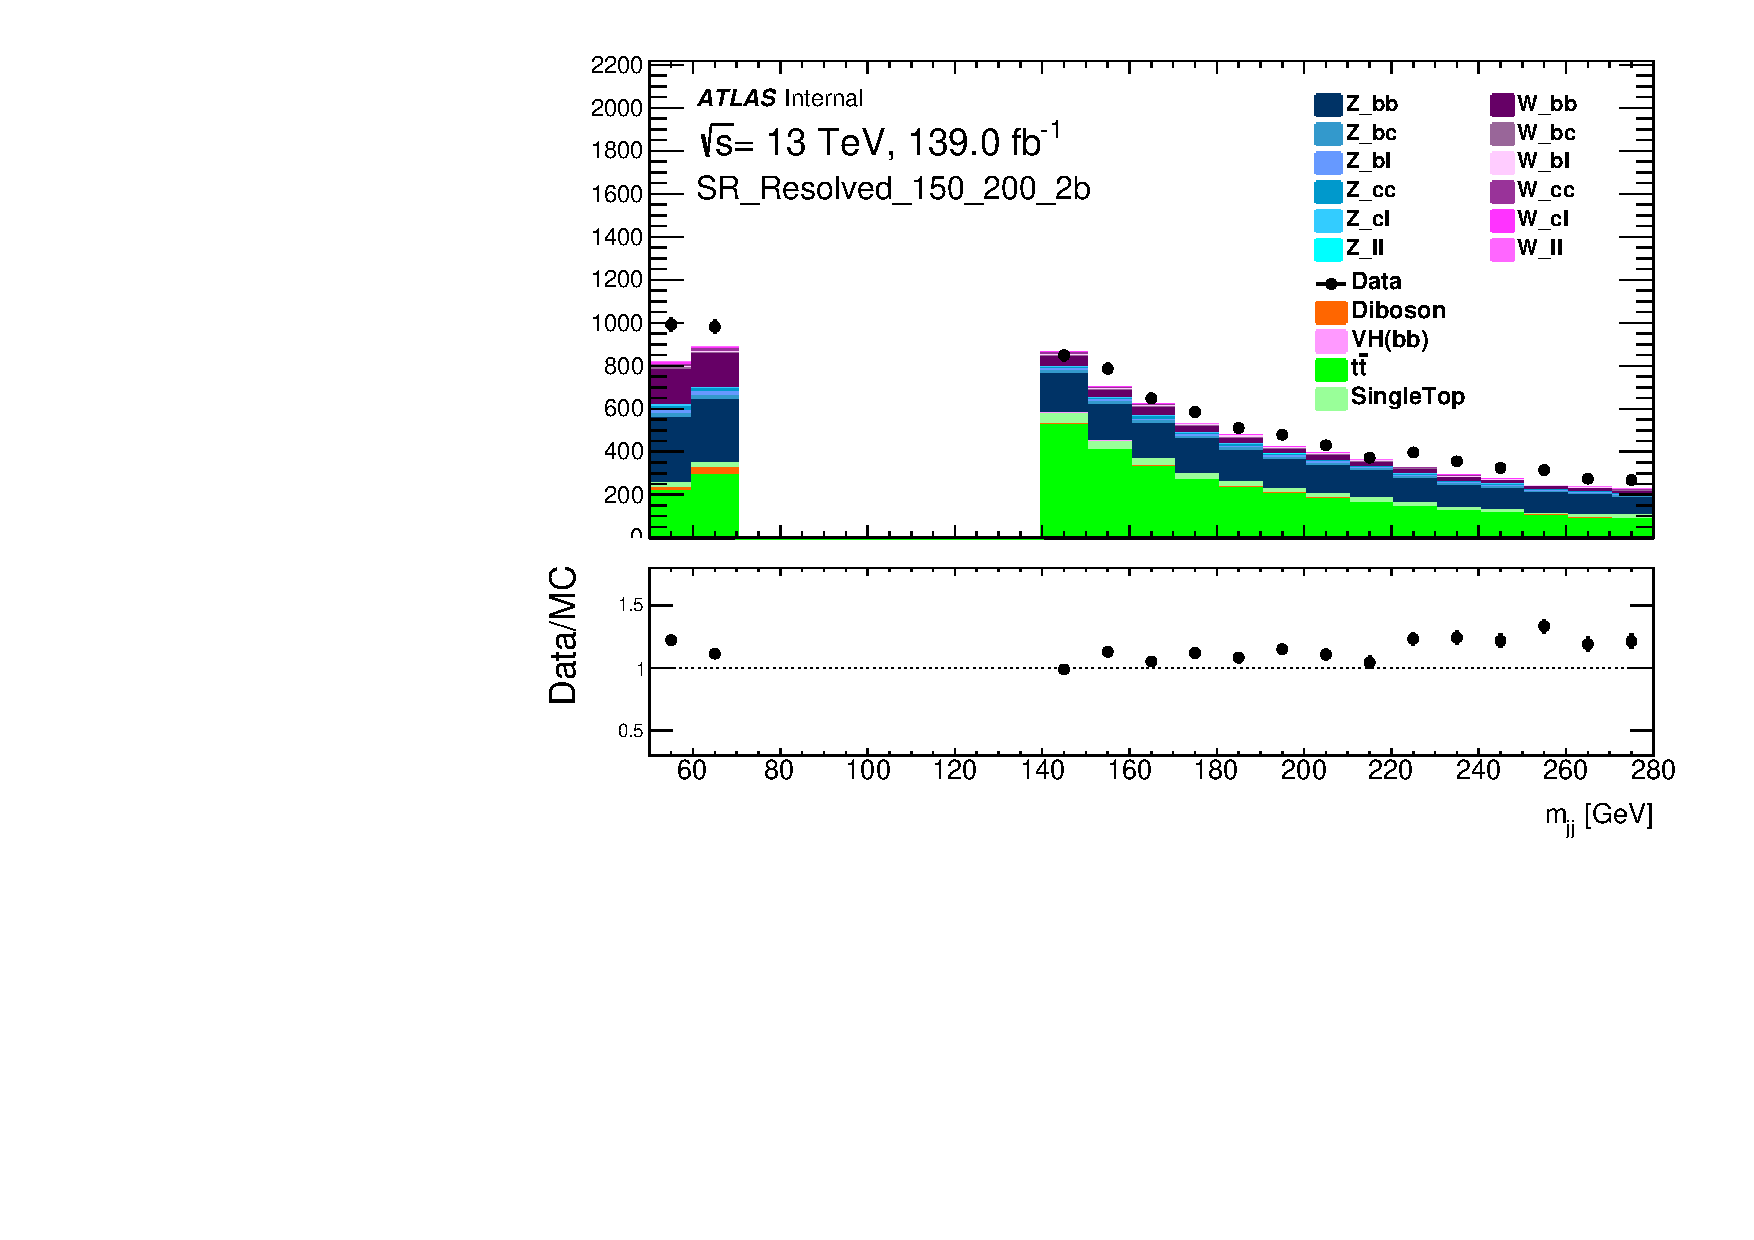
\includegraphics[width=0.46\linewidth]{chapters/c8/figures/0L/DataMC_MonoH_Nominal_SR_Resolved_150_200_2b_m_jj_10GeV.pdf}
    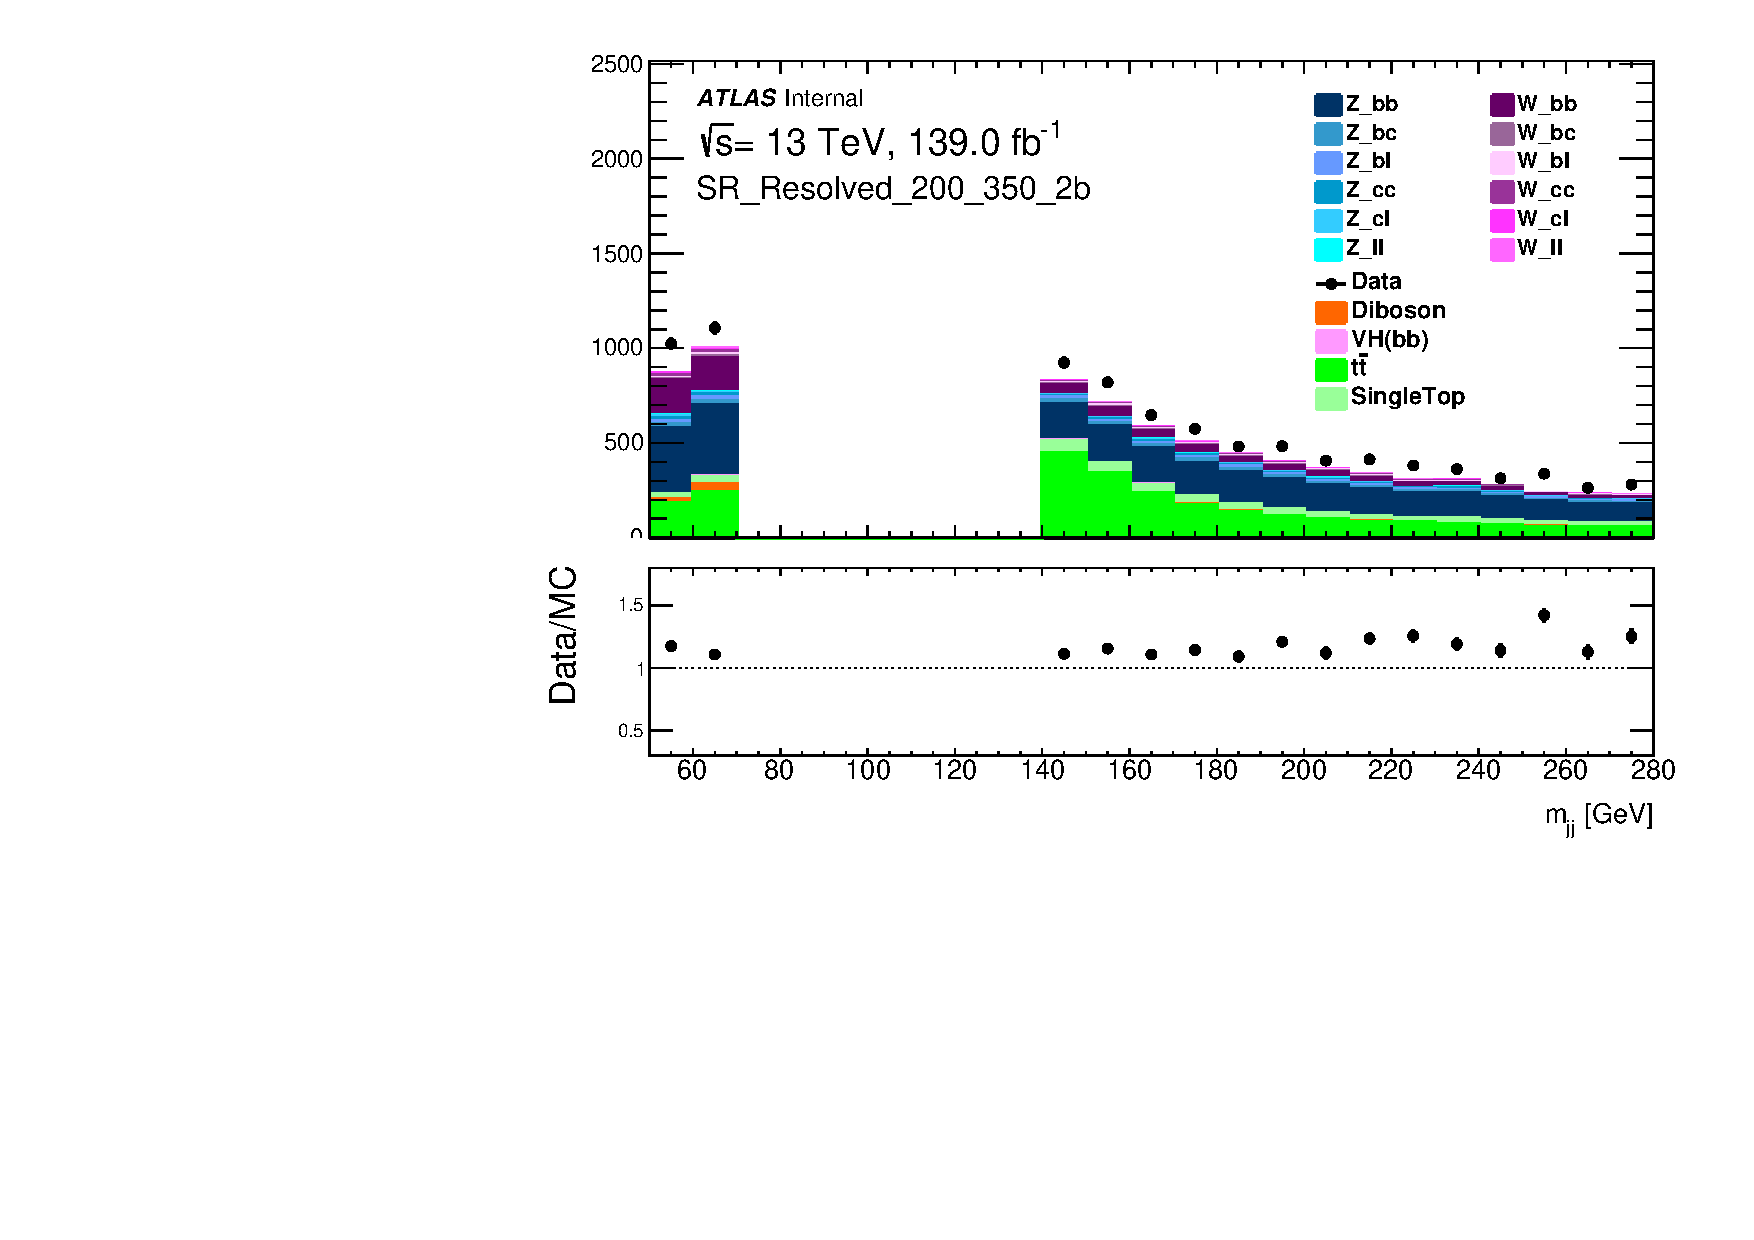
\includegraphics[width=0.46\linewidth]{chapters/c8/figures/0L/DataMC_MonoH_Nominal_SR_Resolved_200_350_2b_m_jj_10GeV.pdf}\\
    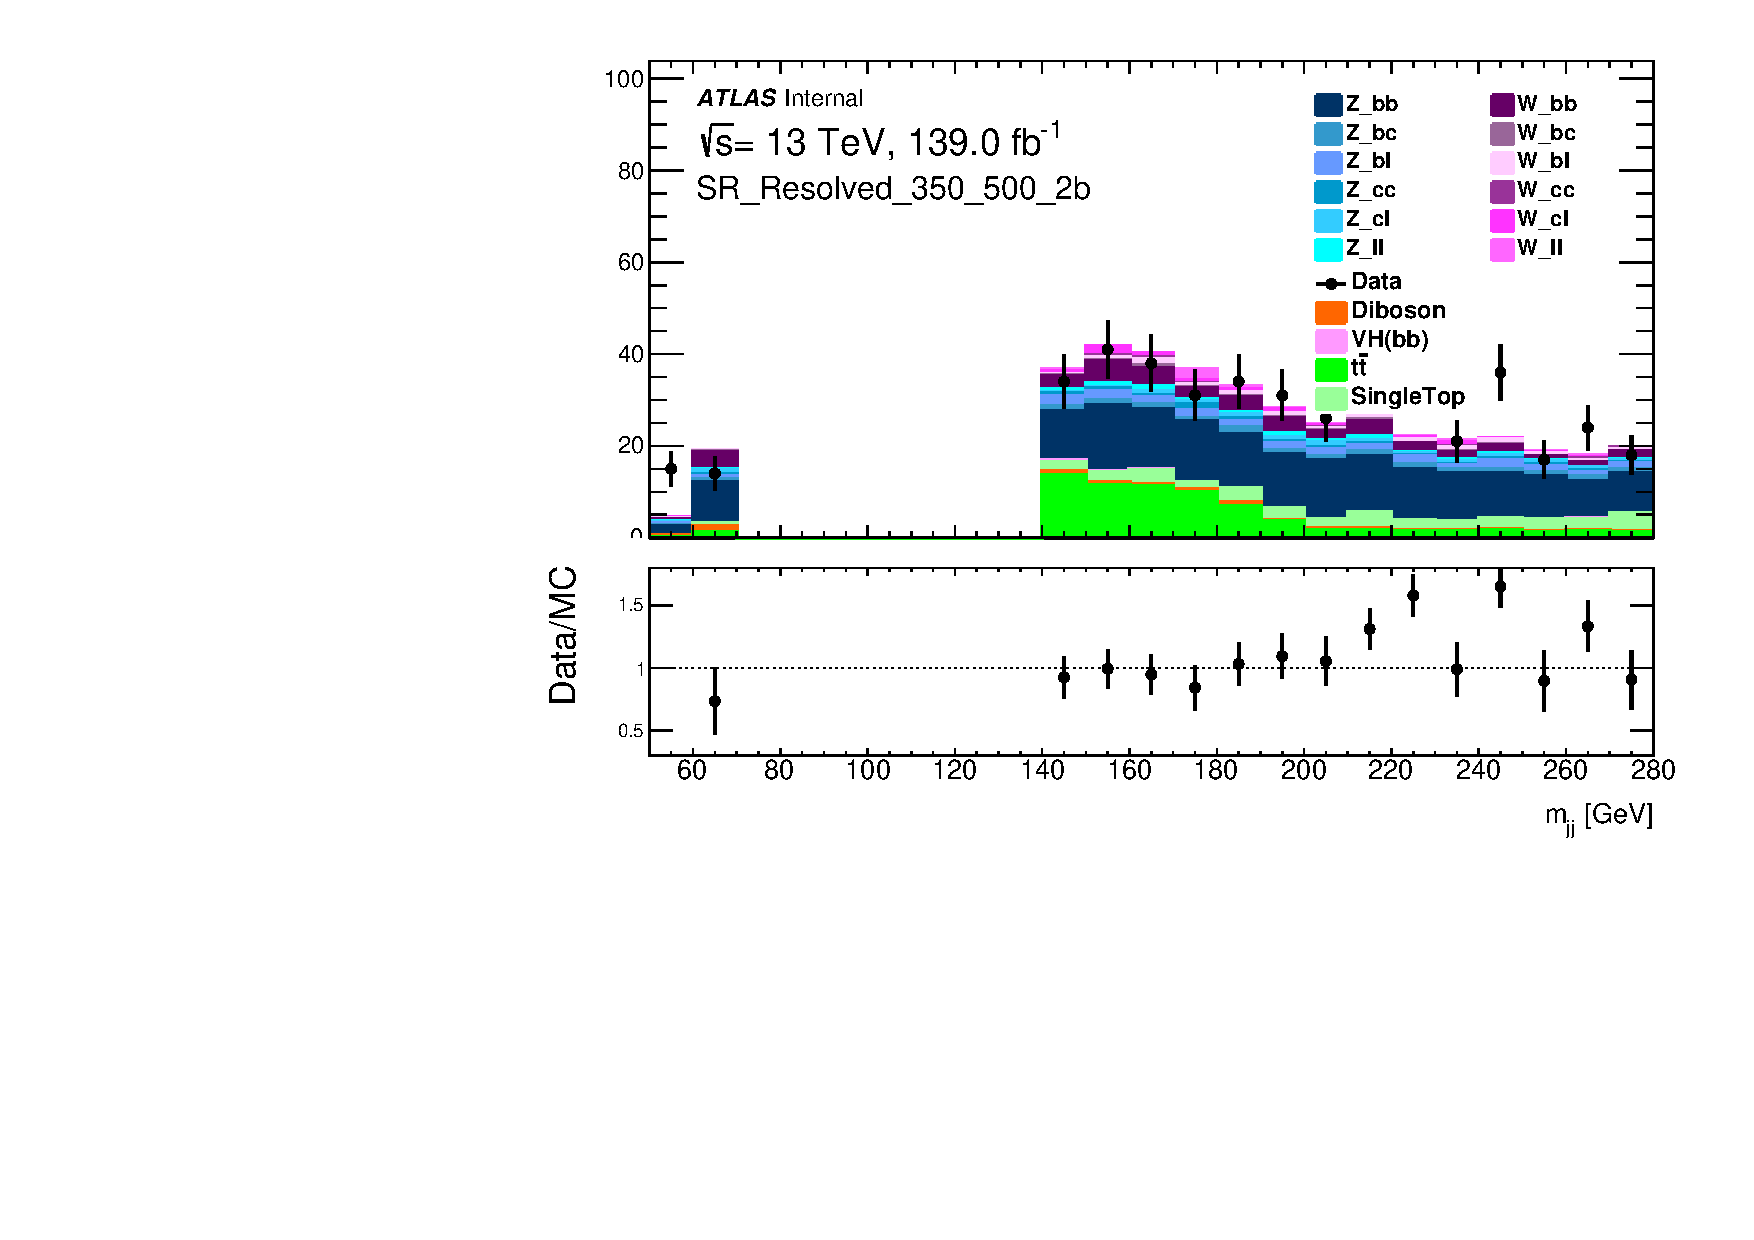
\includegraphics[width=0.46\linewidth]{chapters/c8/figures/0L/DataMC_MonoH_Nominal_SR_Resolved_350_500_2b_m_jj_10GeV.pdf}
    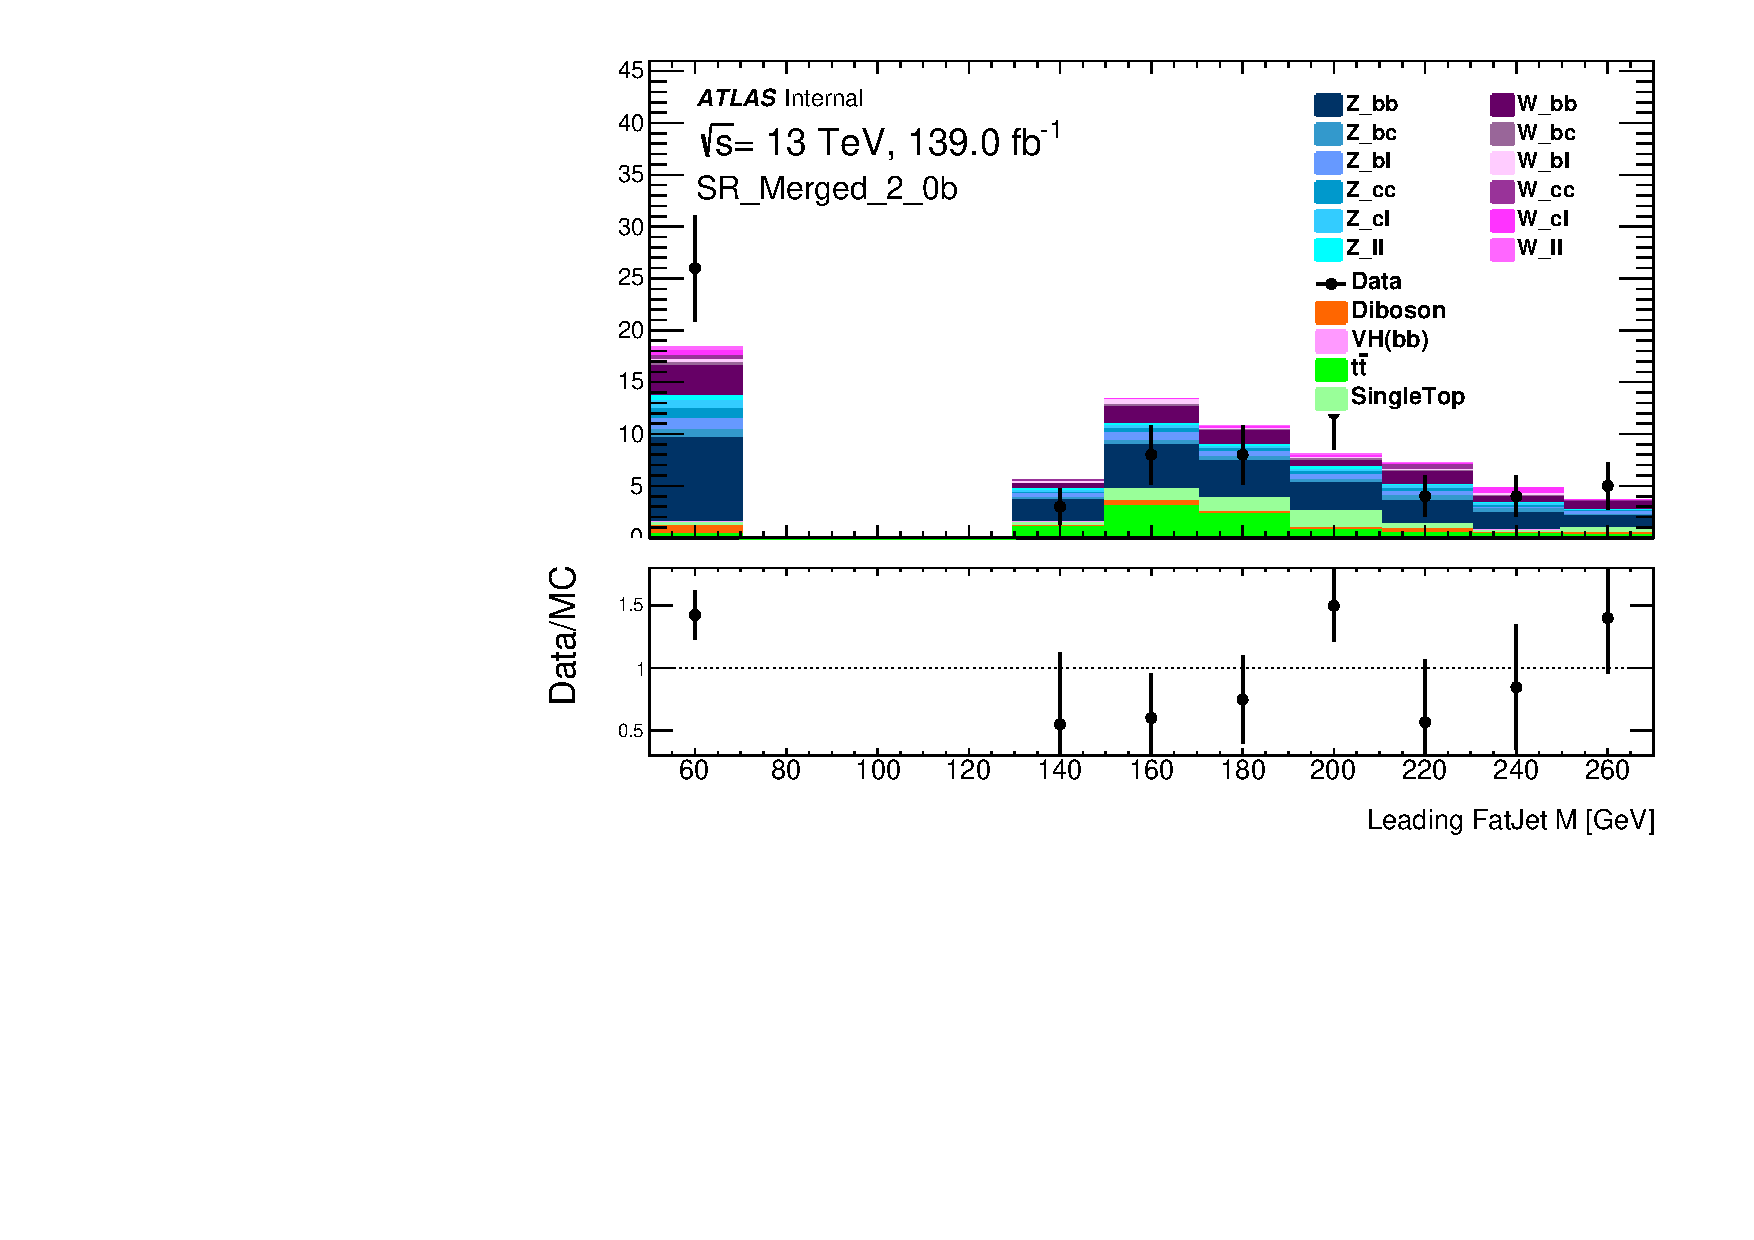
\includegraphics[width=0.46\linewidth]{chapters/c8/figures/0L/DataMC_MonoH_Nominal_SR_Merged_2_0b_fatjets_m1_20GeV.pdf}
    \caption{Higgs candidate mass spectra in the different \met regions with 2 $b$-tagged jets in the 0-lepton channel.}
    \label{fig:data-mc-0l-mjj-2b}
\end{figure}

\begin{figure}[!htb]
    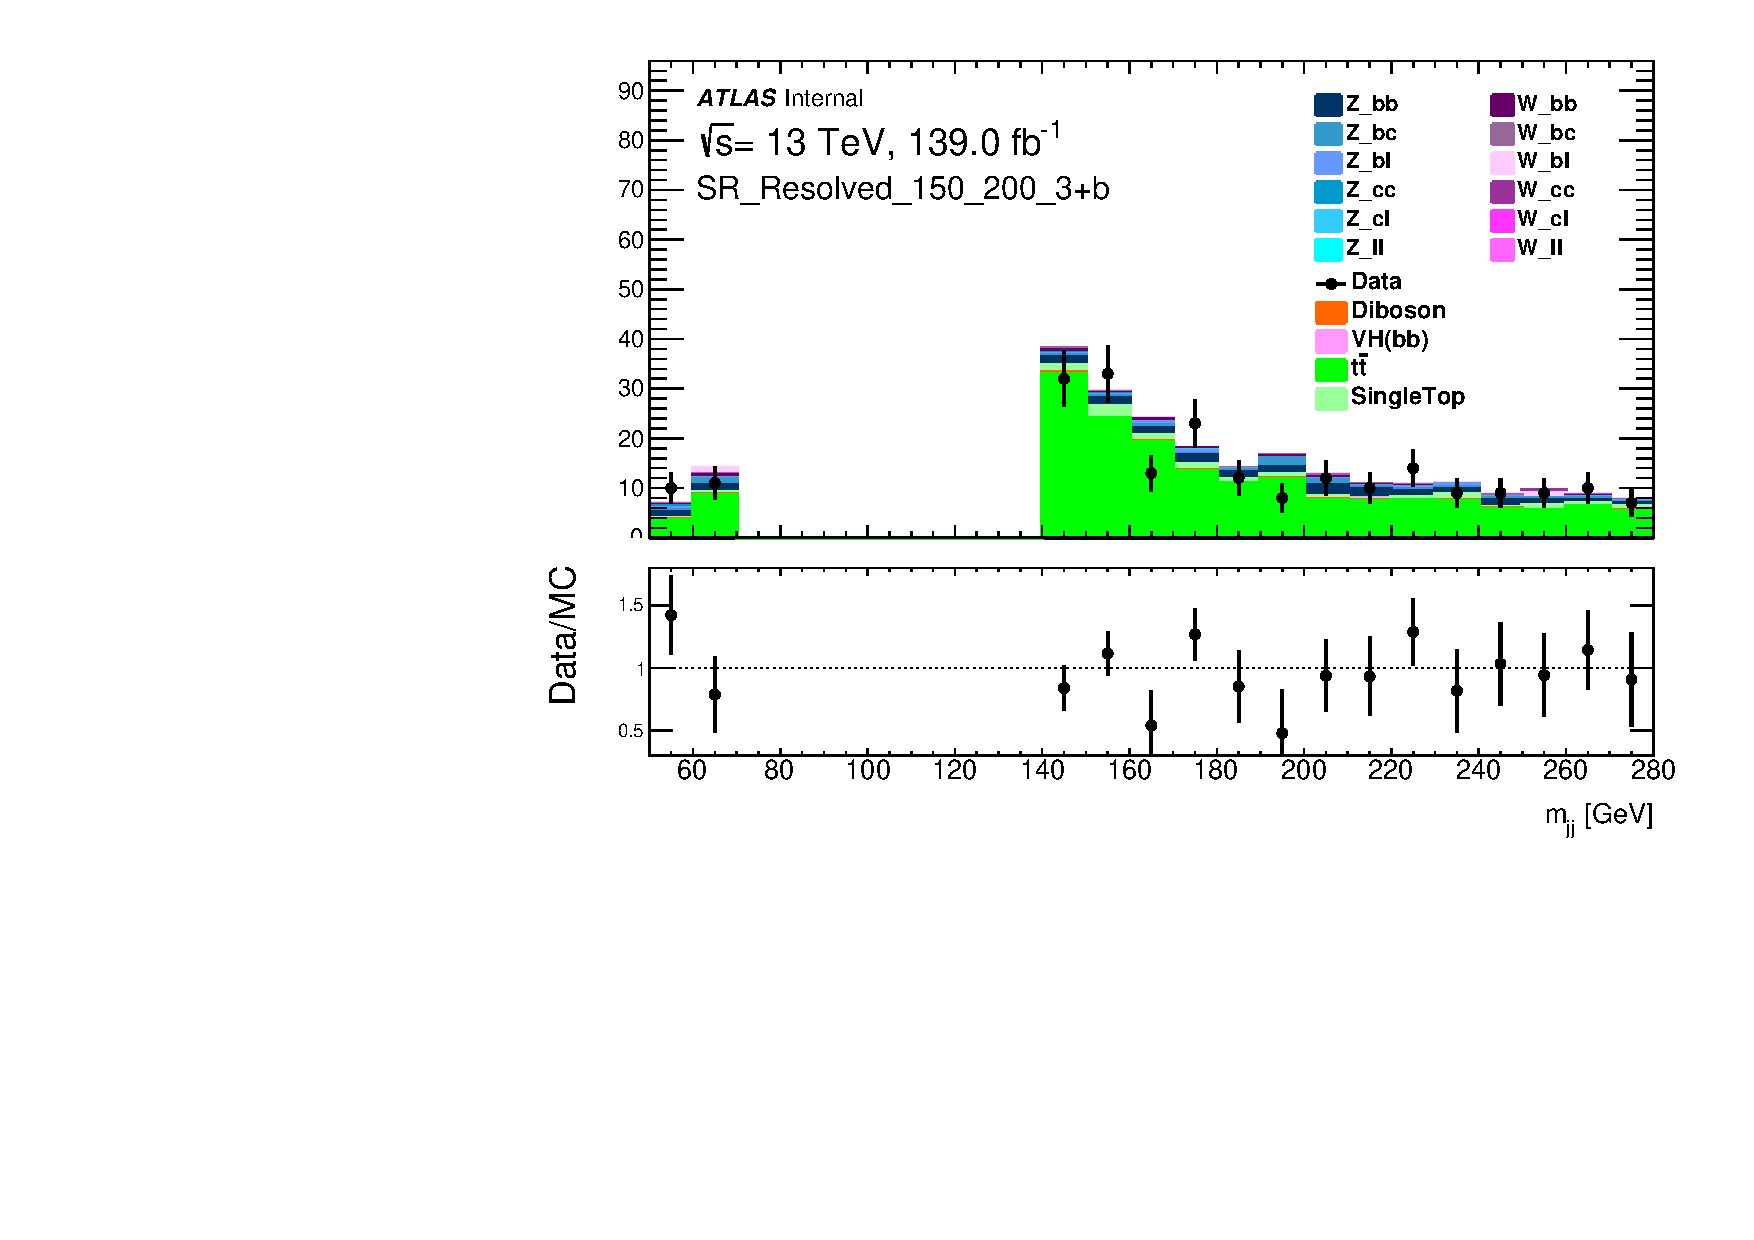
\includegraphics[width=0.46\linewidth]{chapters/c8/figures/0L/DataMC_MonoH_Nominal_SR_Resolved_150_200_3+b_m_jj_10GeV.pdf}
    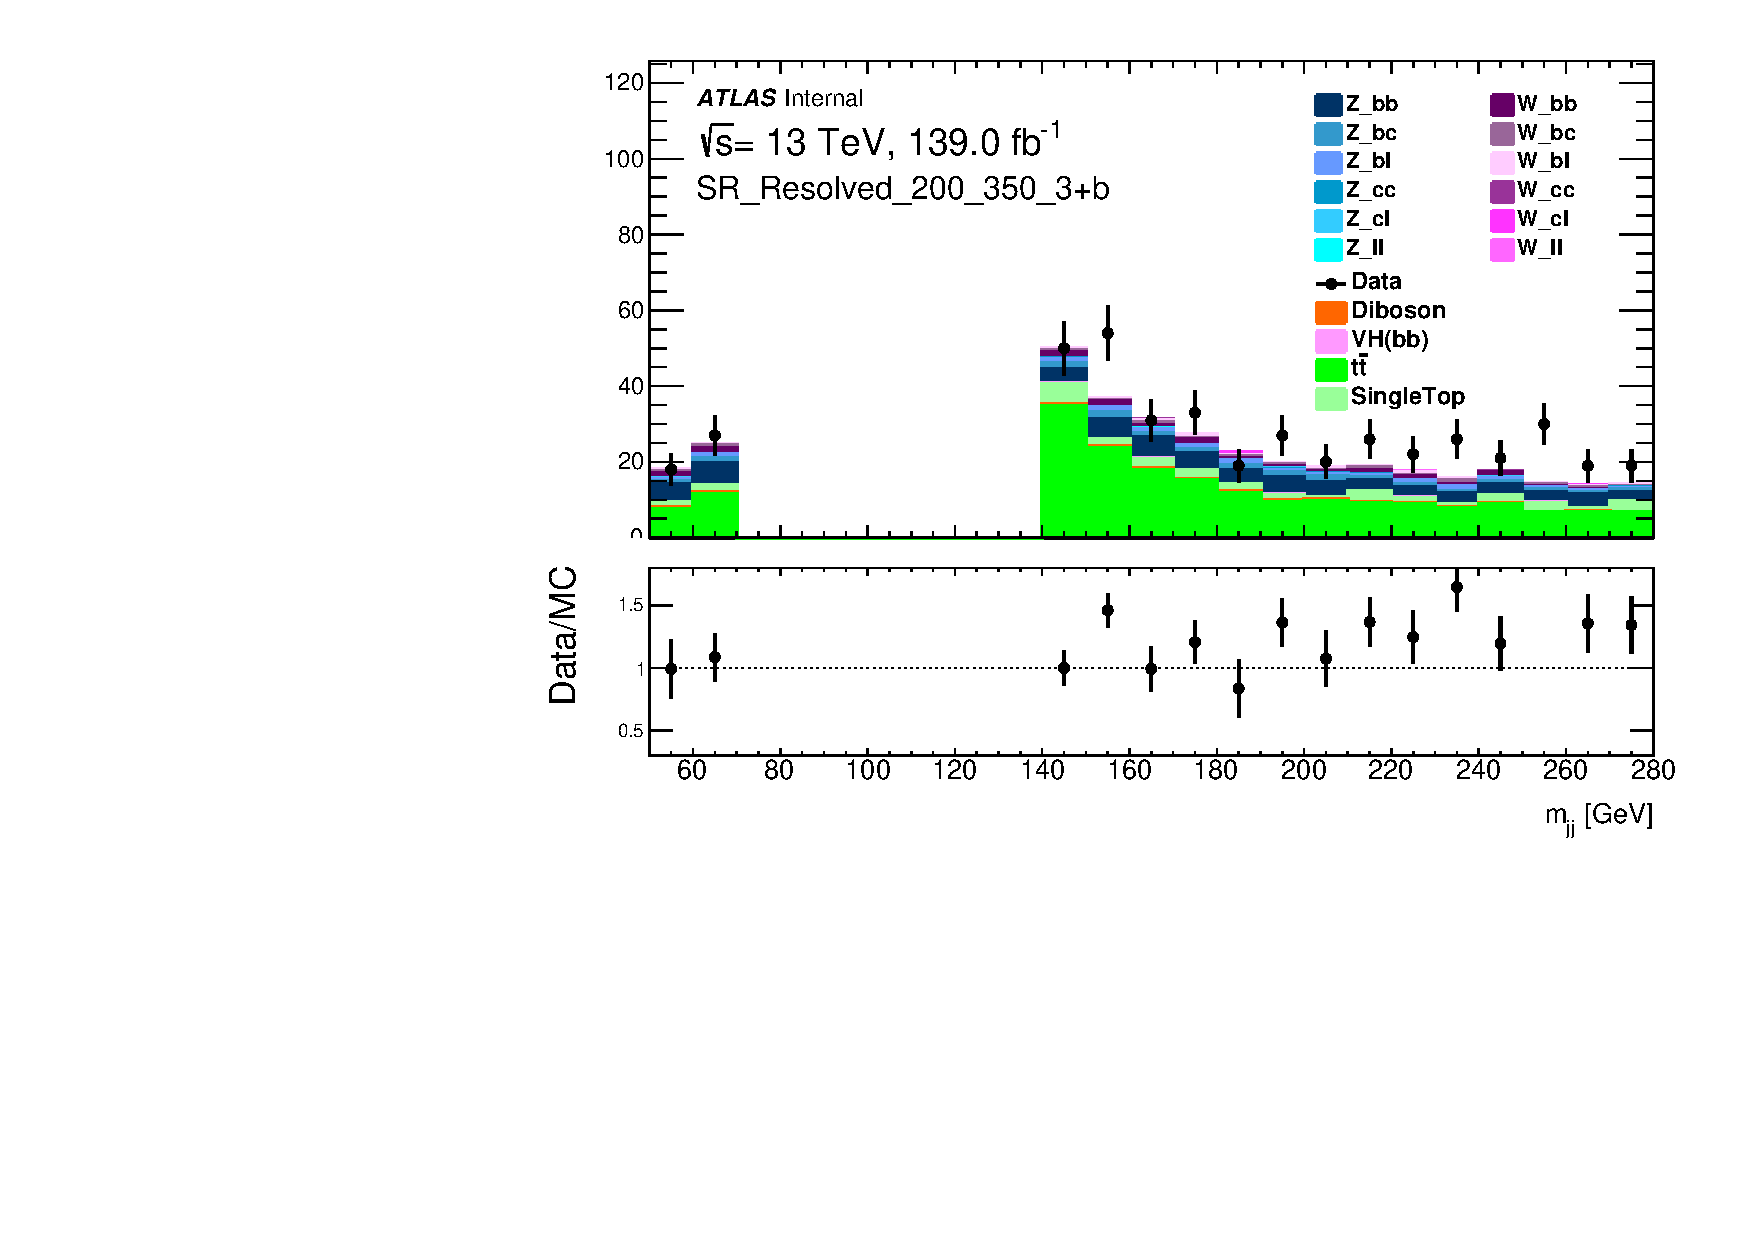
\includegraphics[width=0.46\linewidth]{chapters/c8/figures/0L/DataMC_MonoH_Nominal_SR_Resolved_200_350_3+b_m_jj_10GeV.pdf}\\
    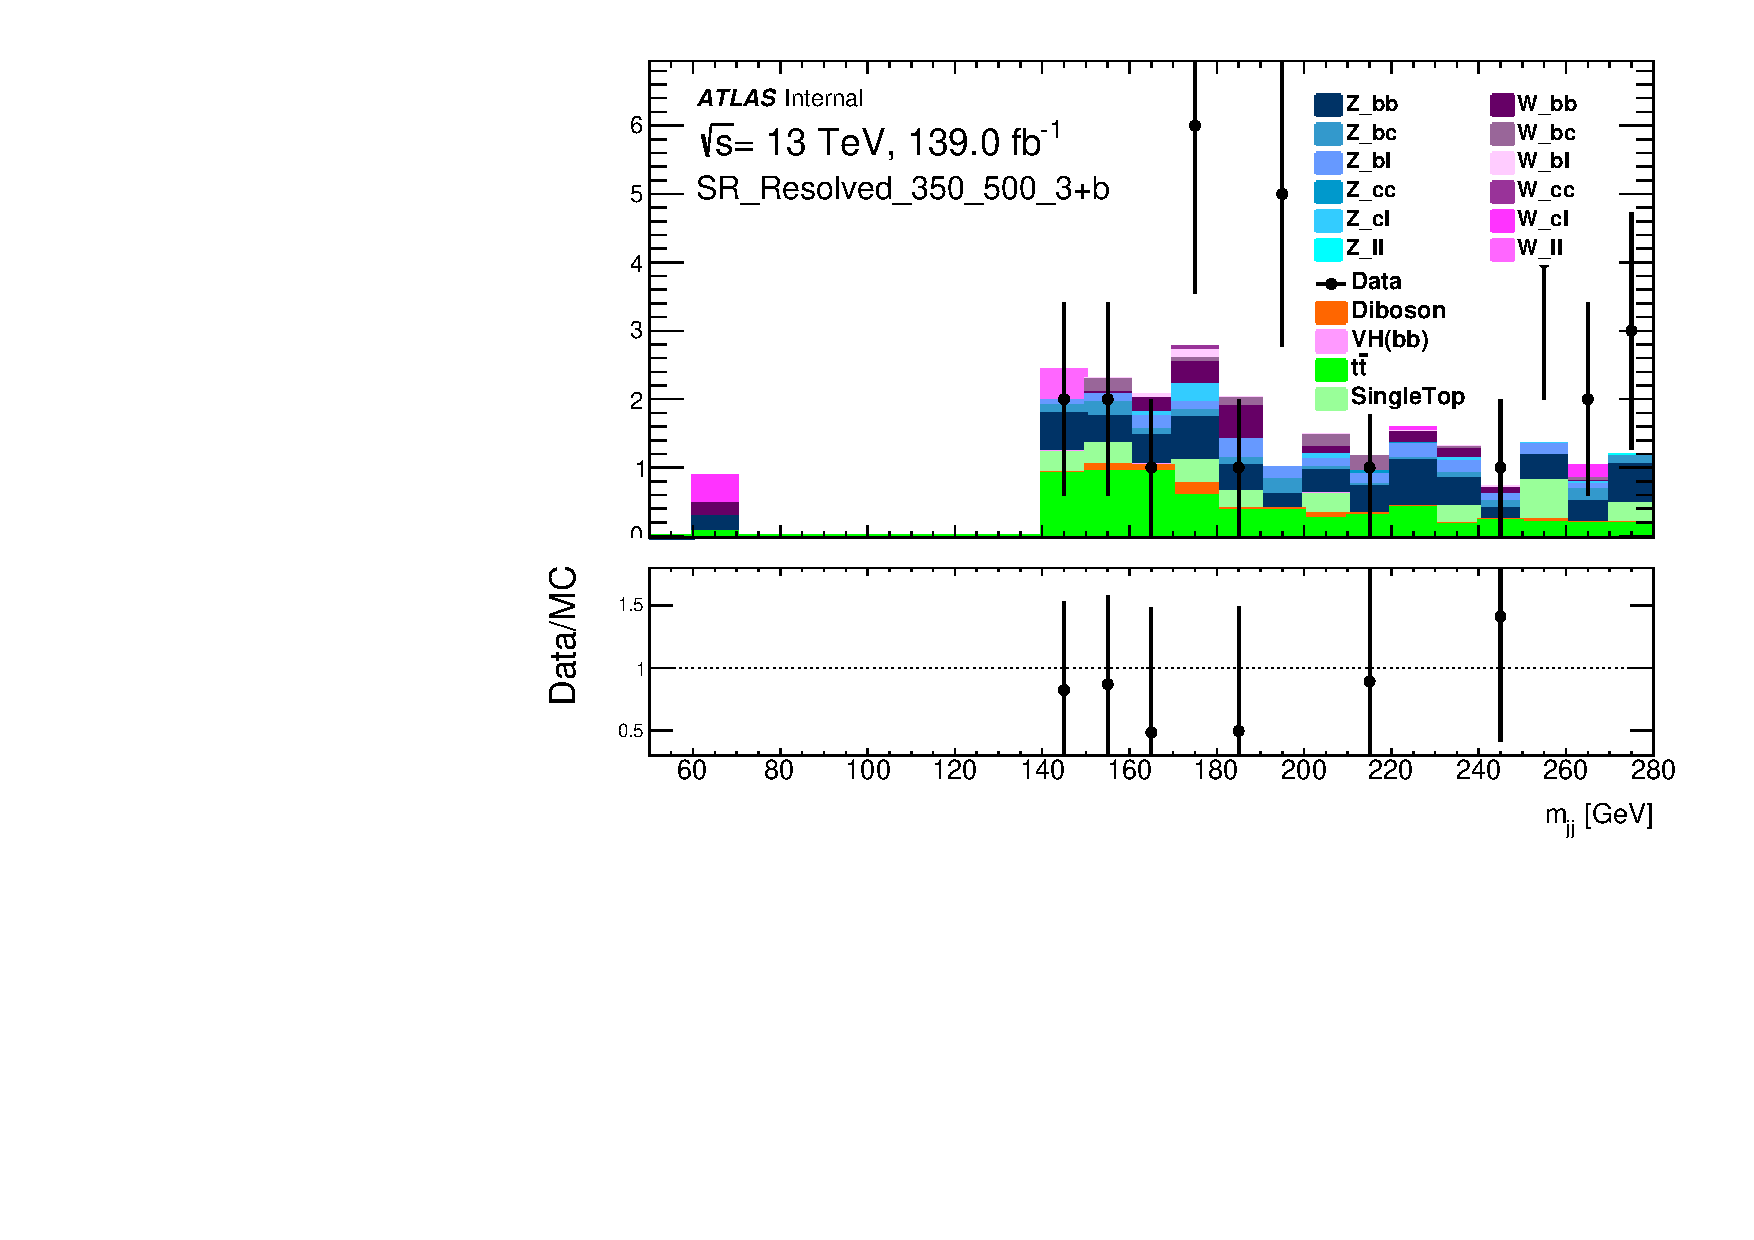
\includegraphics[width=0.46\linewidth]{chapters/c8/figures/0L/DataMC_MonoH_Nominal_SR_Resolved_350_500_3+b_m_jj_10GeV.pdf}
    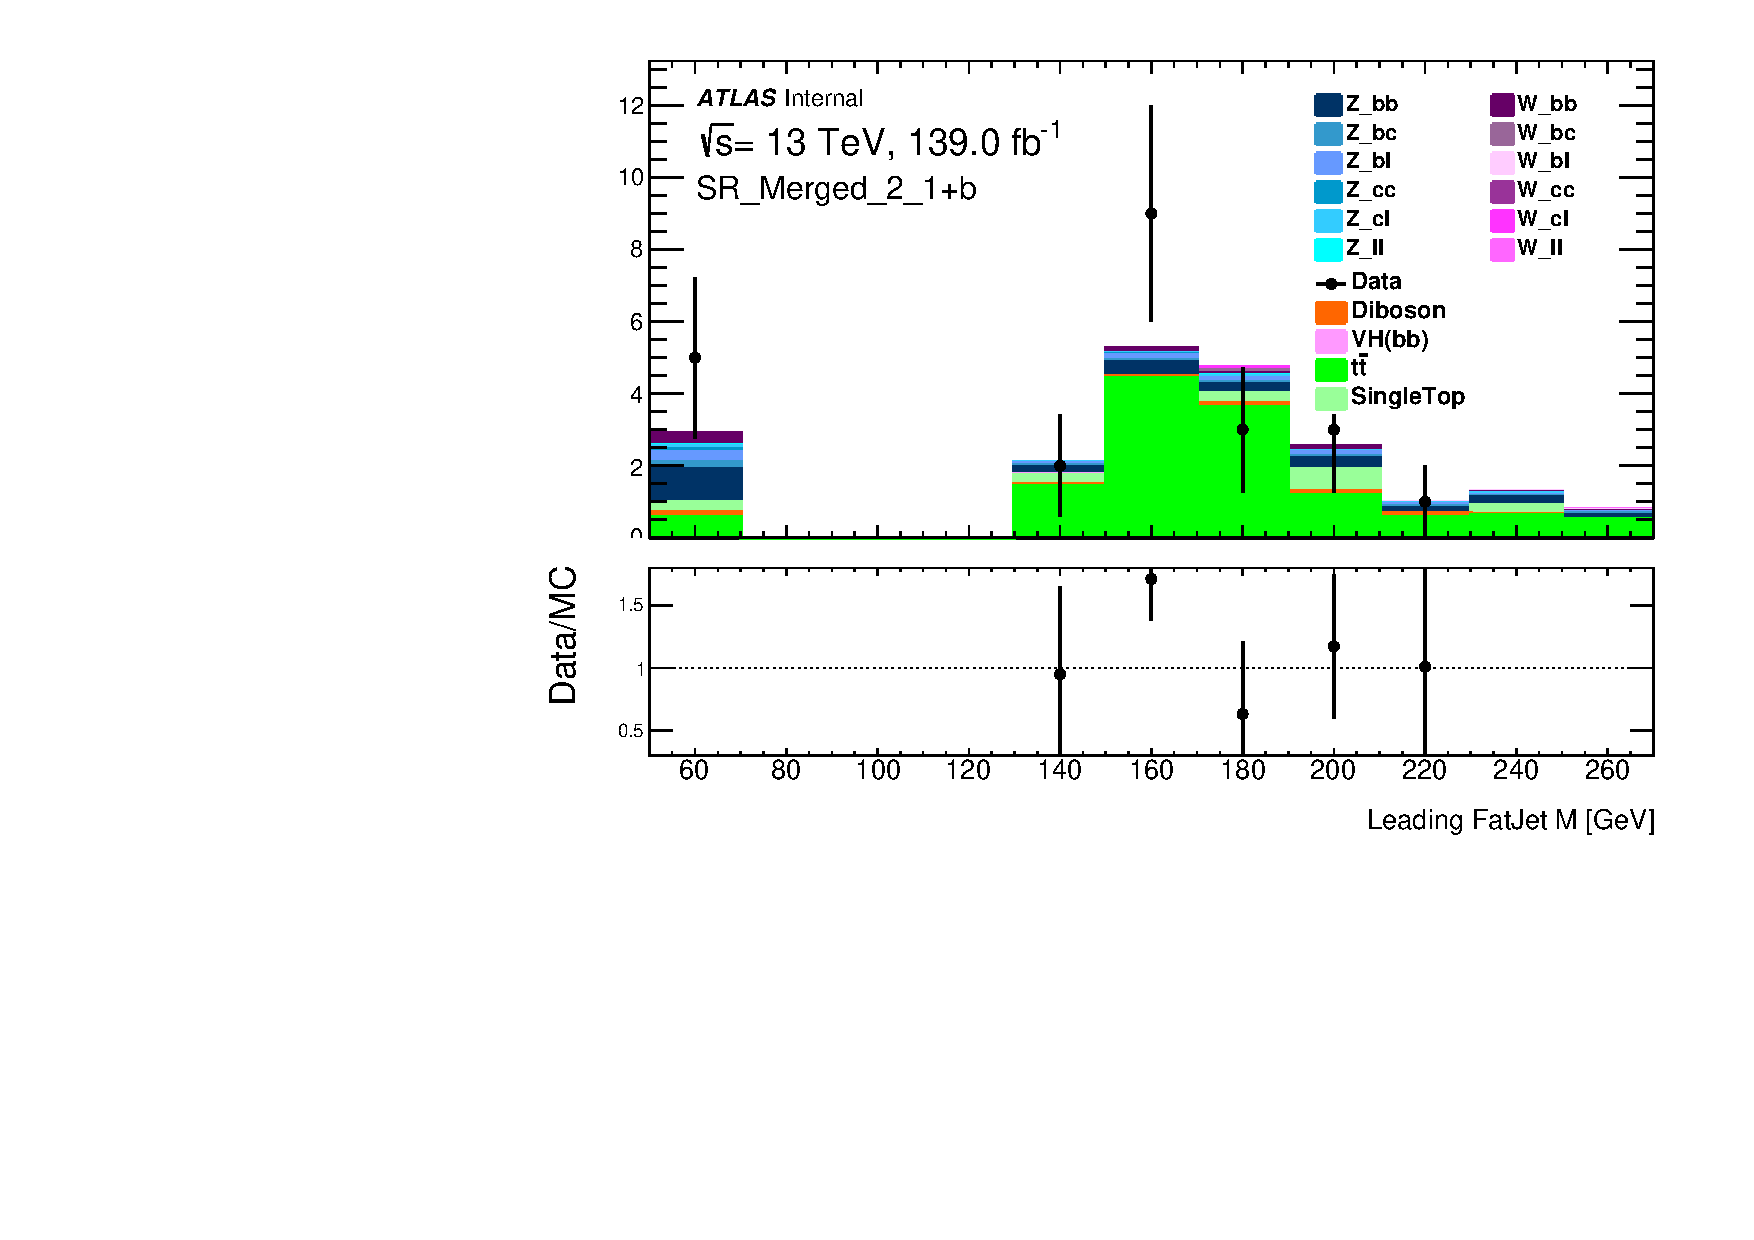
\includegraphics[width=0.46\linewidth]{chapters/c8/figures/0L/DataMC_MonoH_Nominal_SR_Merged_2_1+b_fatjets_m1_20GeV.pdf}
    \caption{Higgs candidate mass spectra in the different \met regions with at least 3 $b$-tagged jets in the 0-lepton channel.}
    \label{fig:data-mc-0l-mjj-3+b}
\end{figure}

\begin{figure}[!htb]
    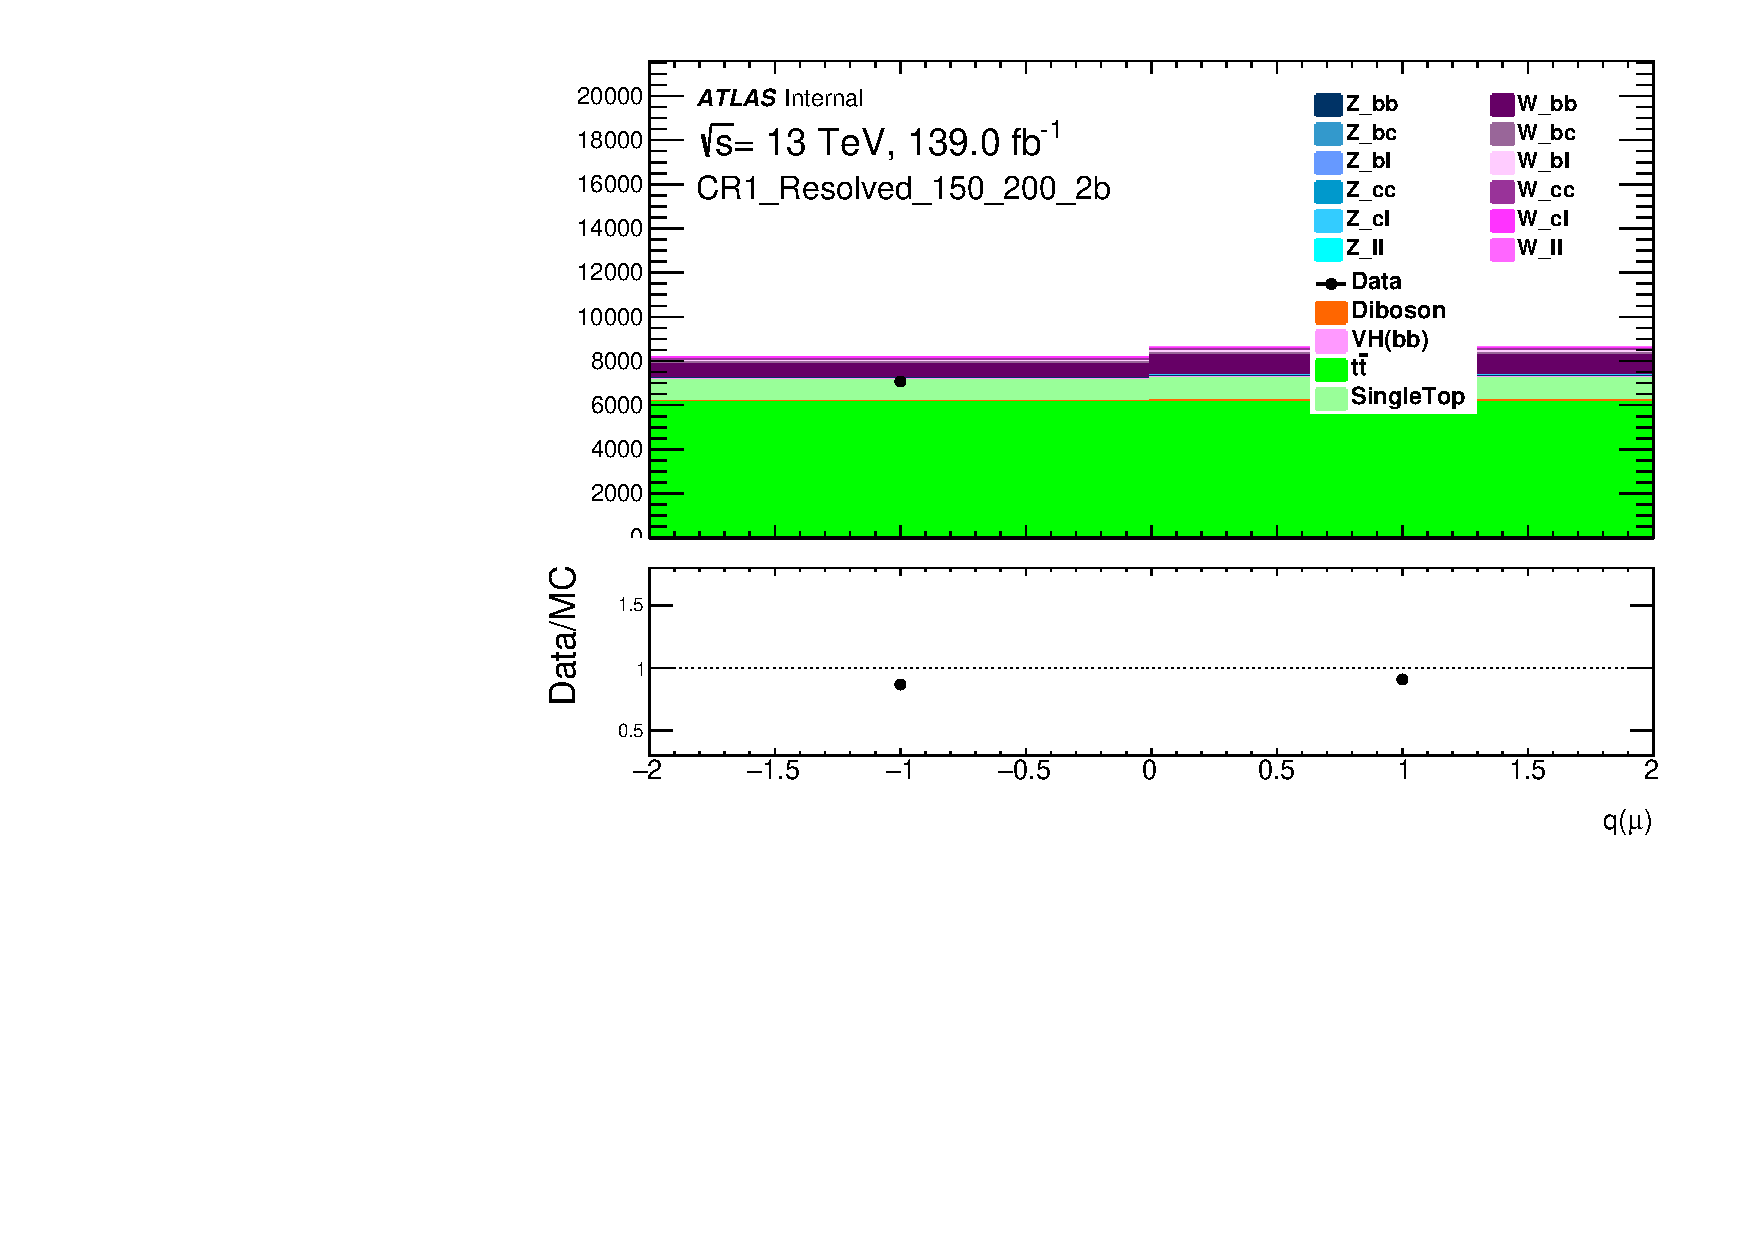
\includegraphics[width=0.46\linewidth]{chapters/c8/figures/1L/DataMC_MonoH_Nominal_CR1_Resolved_150_200_2b_mu_charge.pdf}
    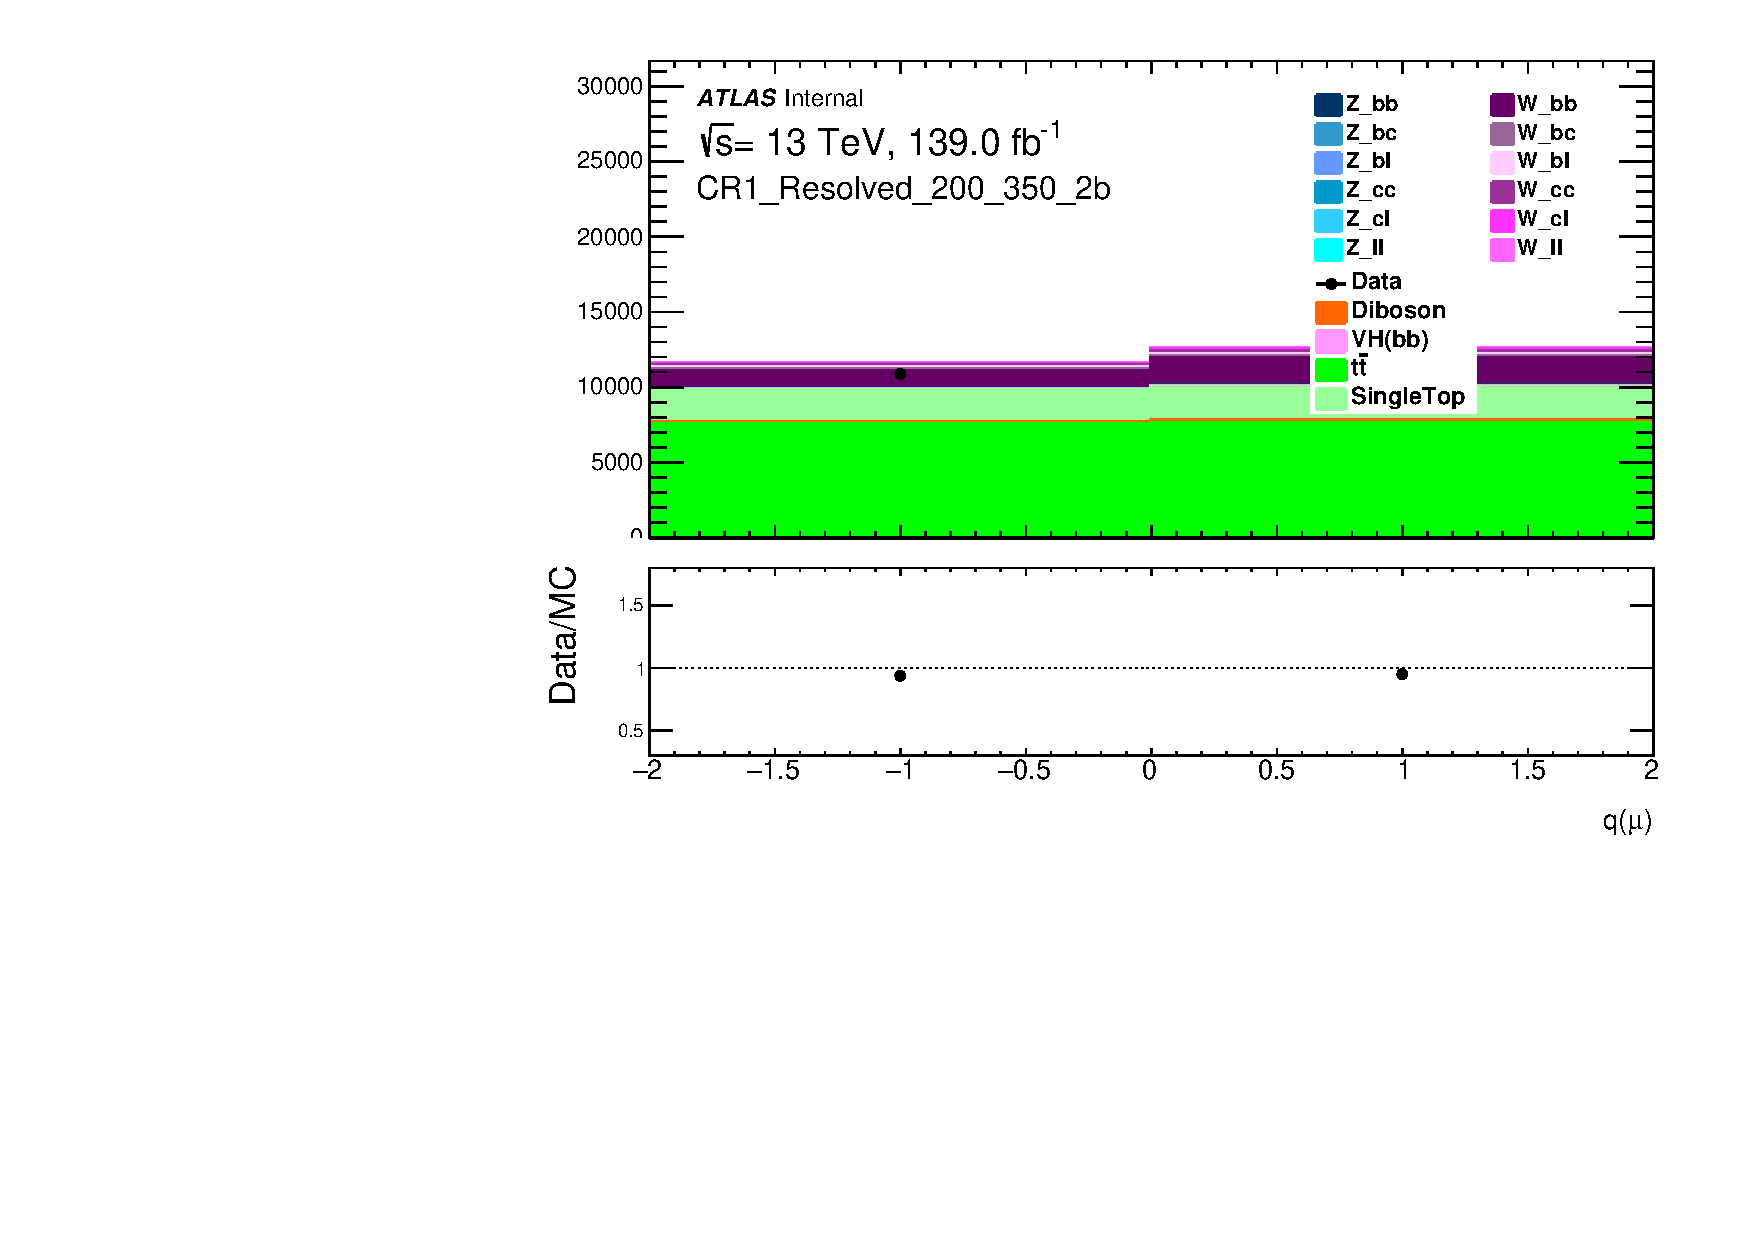
\includegraphics[width=0.46\linewidth]{chapters/c8/figures/1L/DataMC_MonoH_Nominal_CR1_Resolved_200_350_2b_mu_charge.pdf}\\
    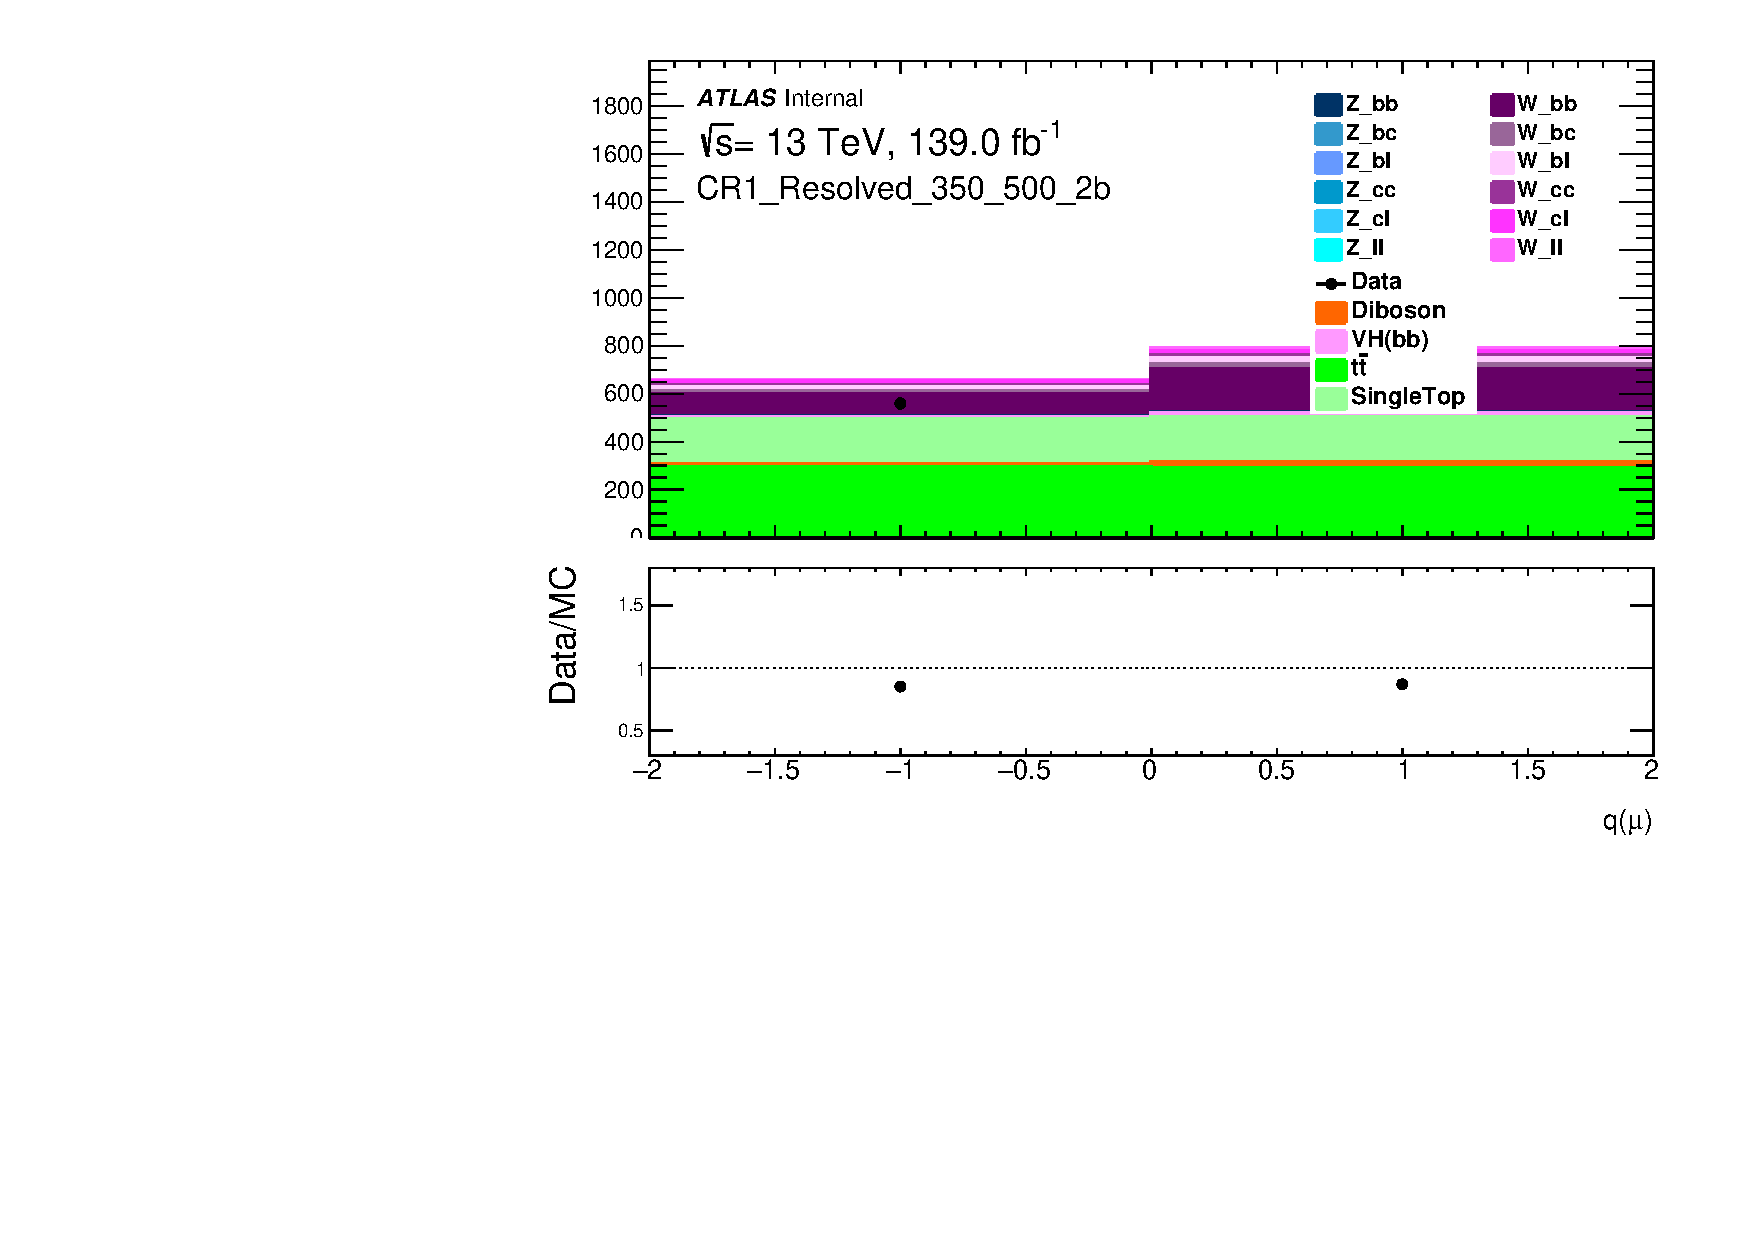
\includegraphics[width=0.46\linewidth]{chapters/c8/figures/1L/DataMC_MonoH_Nominal_CR1_Resolved_350_500_2b_mu_charge.pdf}
    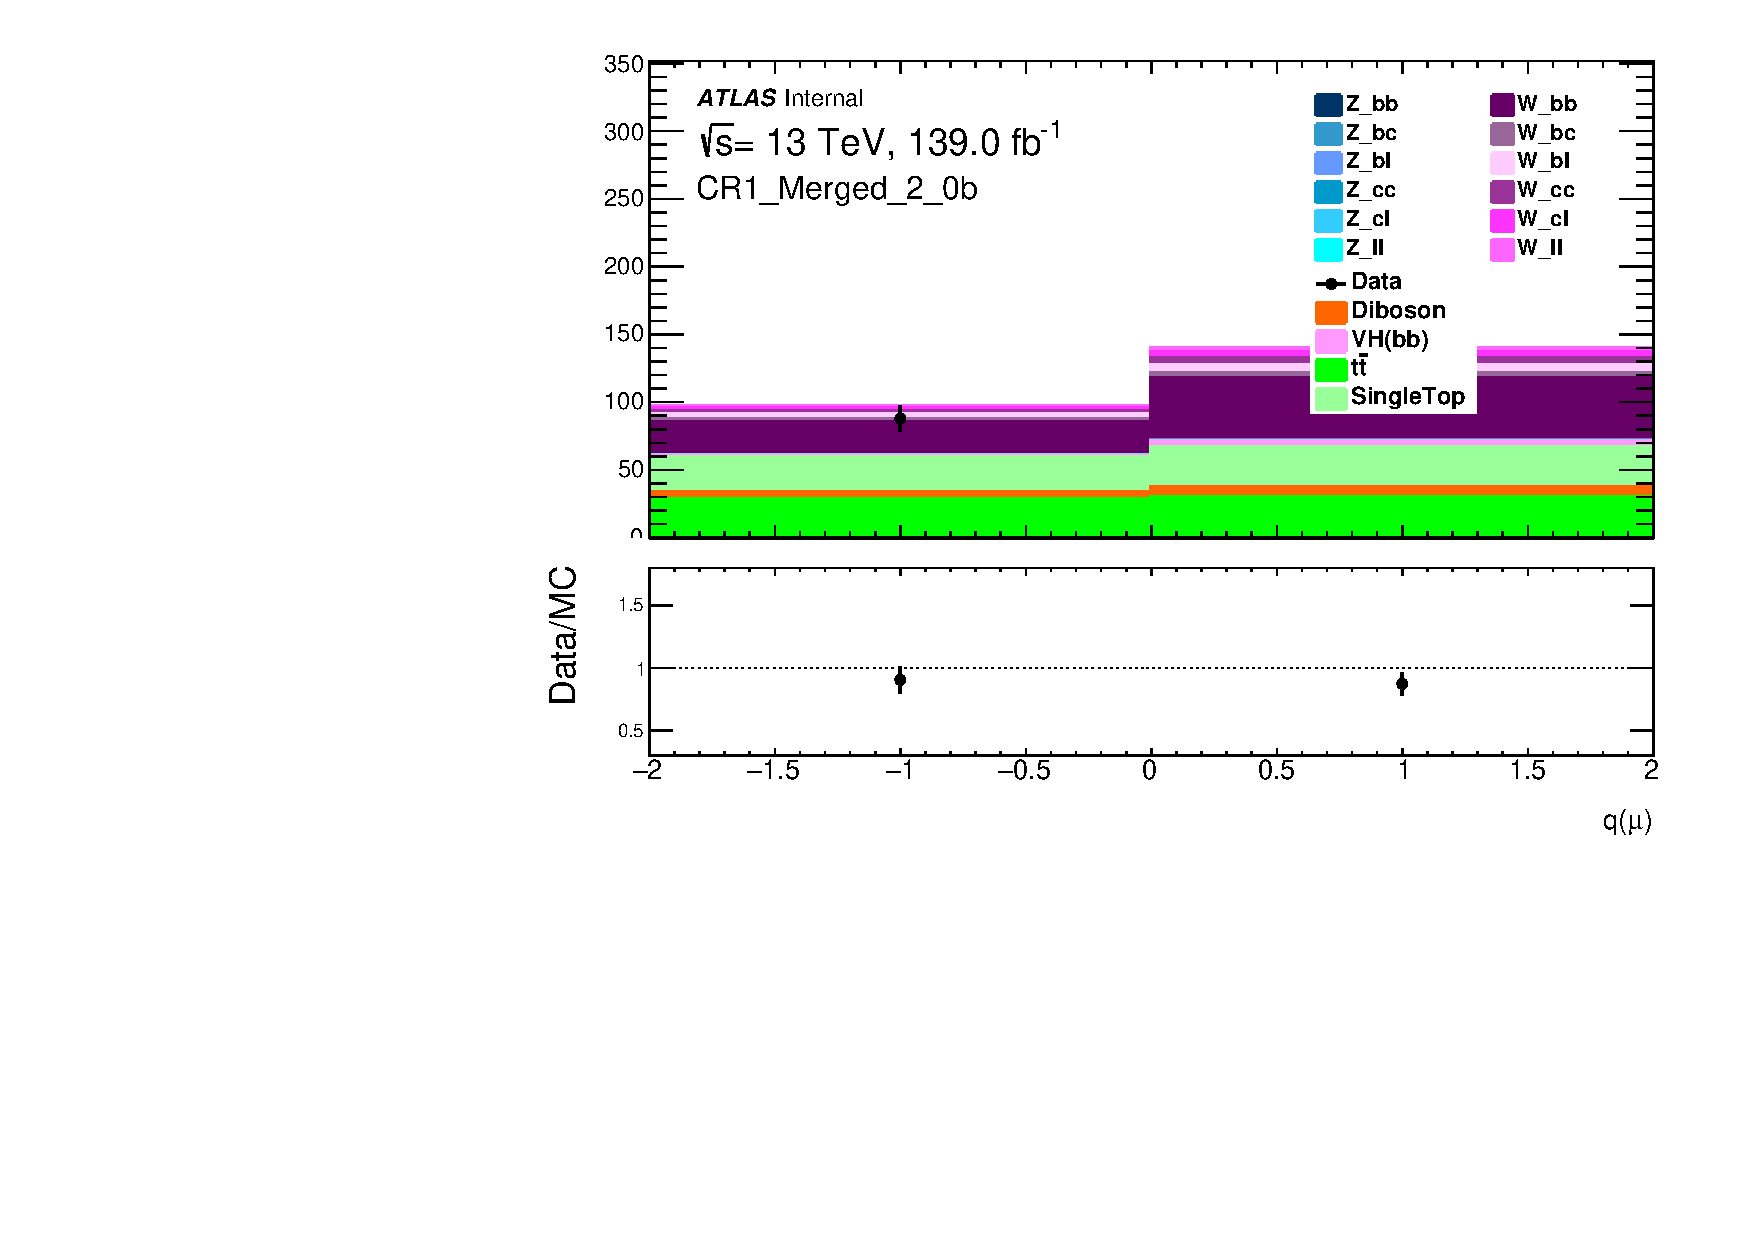
\includegraphics[width=0.46\linewidth]{chapters/c8/figures/1L/DataMC_MonoH_Nominal_CR1_Merged_2_0b_mu_charge.pdf}
    \caption{Muon charge distribution in the different \met regions with 2 $b$-tagged jets in the 1-lepton channel.}
    \label{fig:data-mc-1l-mu-charge-2b}
\end{figure}

\begin{figure}[!htb]
    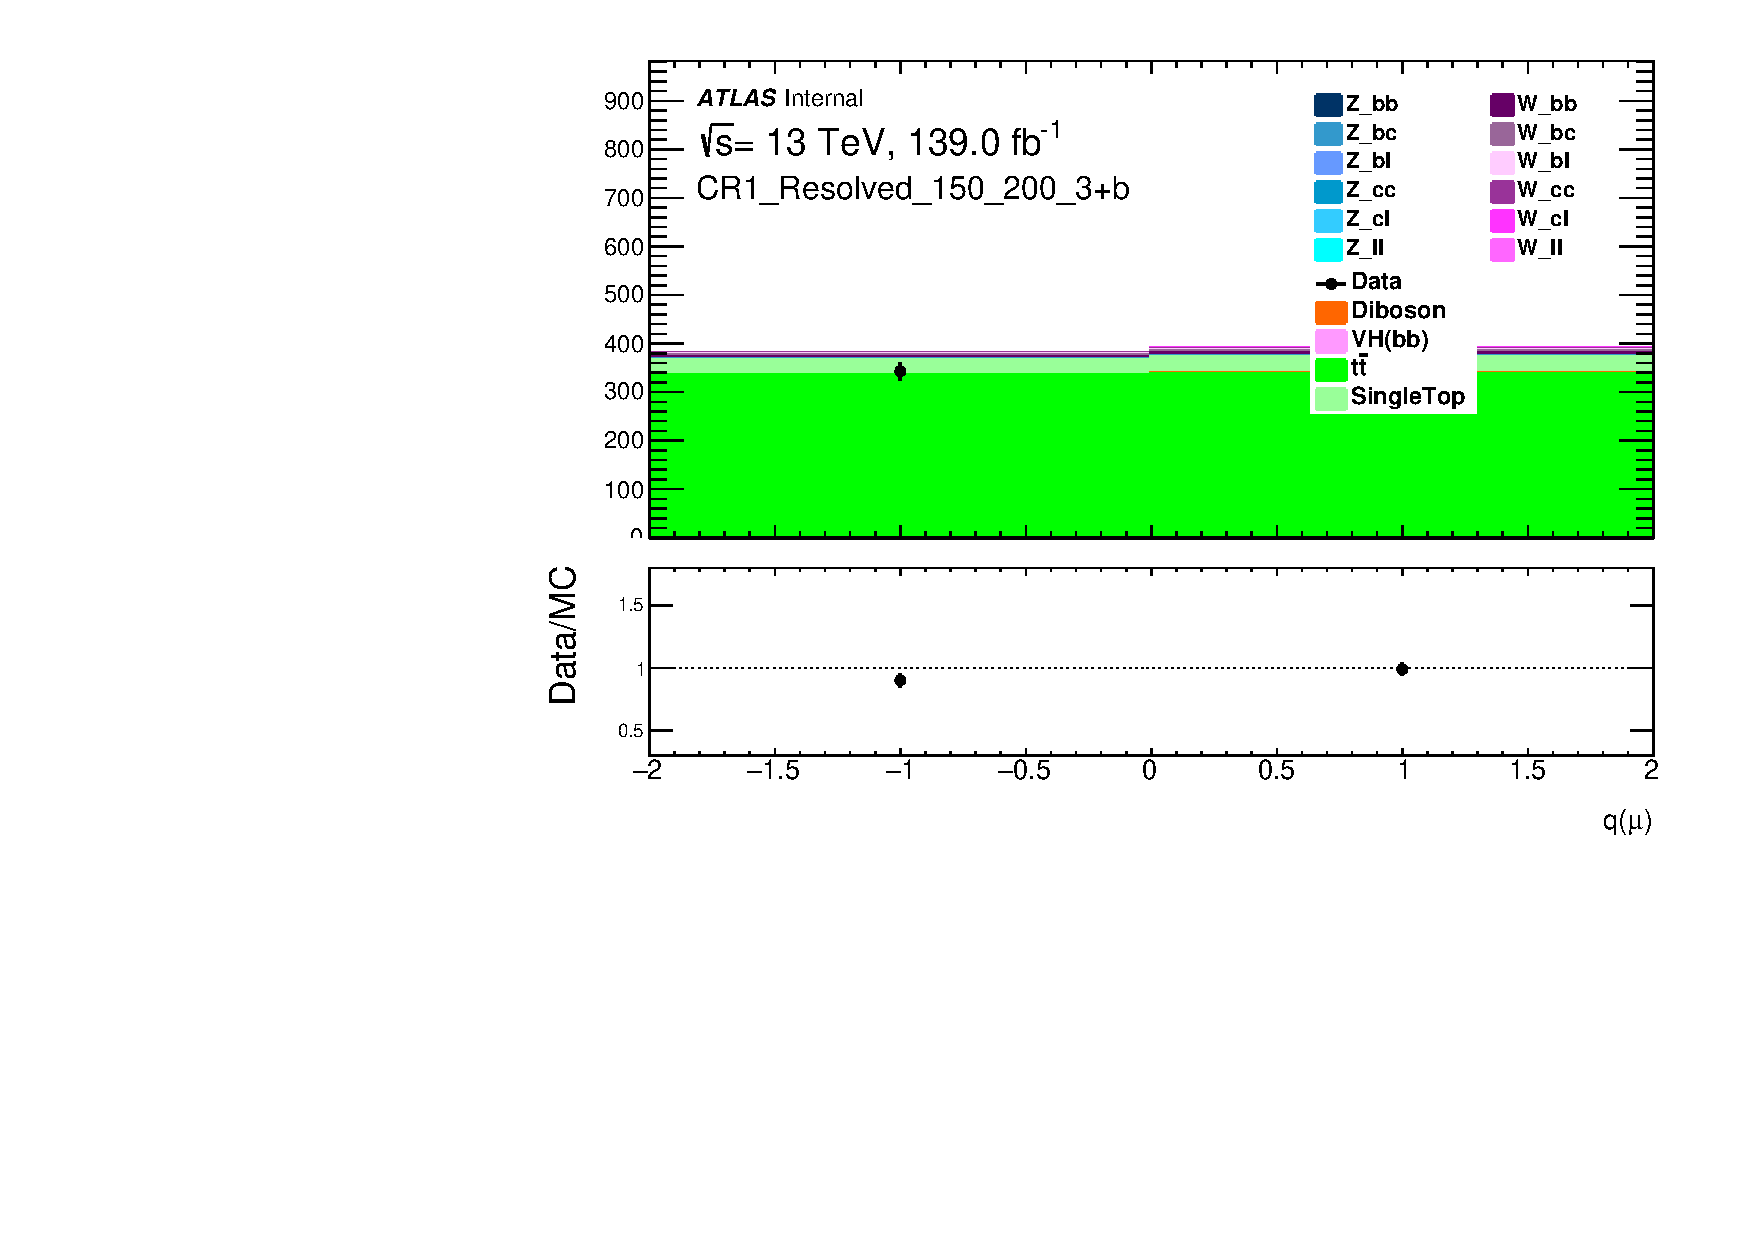
\includegraphics[width=0.46\linewidth]{chapters/c8/figures/1L/DataMC_MonoH_Nominal_CR1_Resolved_150_200_3+b_mu_charge.pdf}
    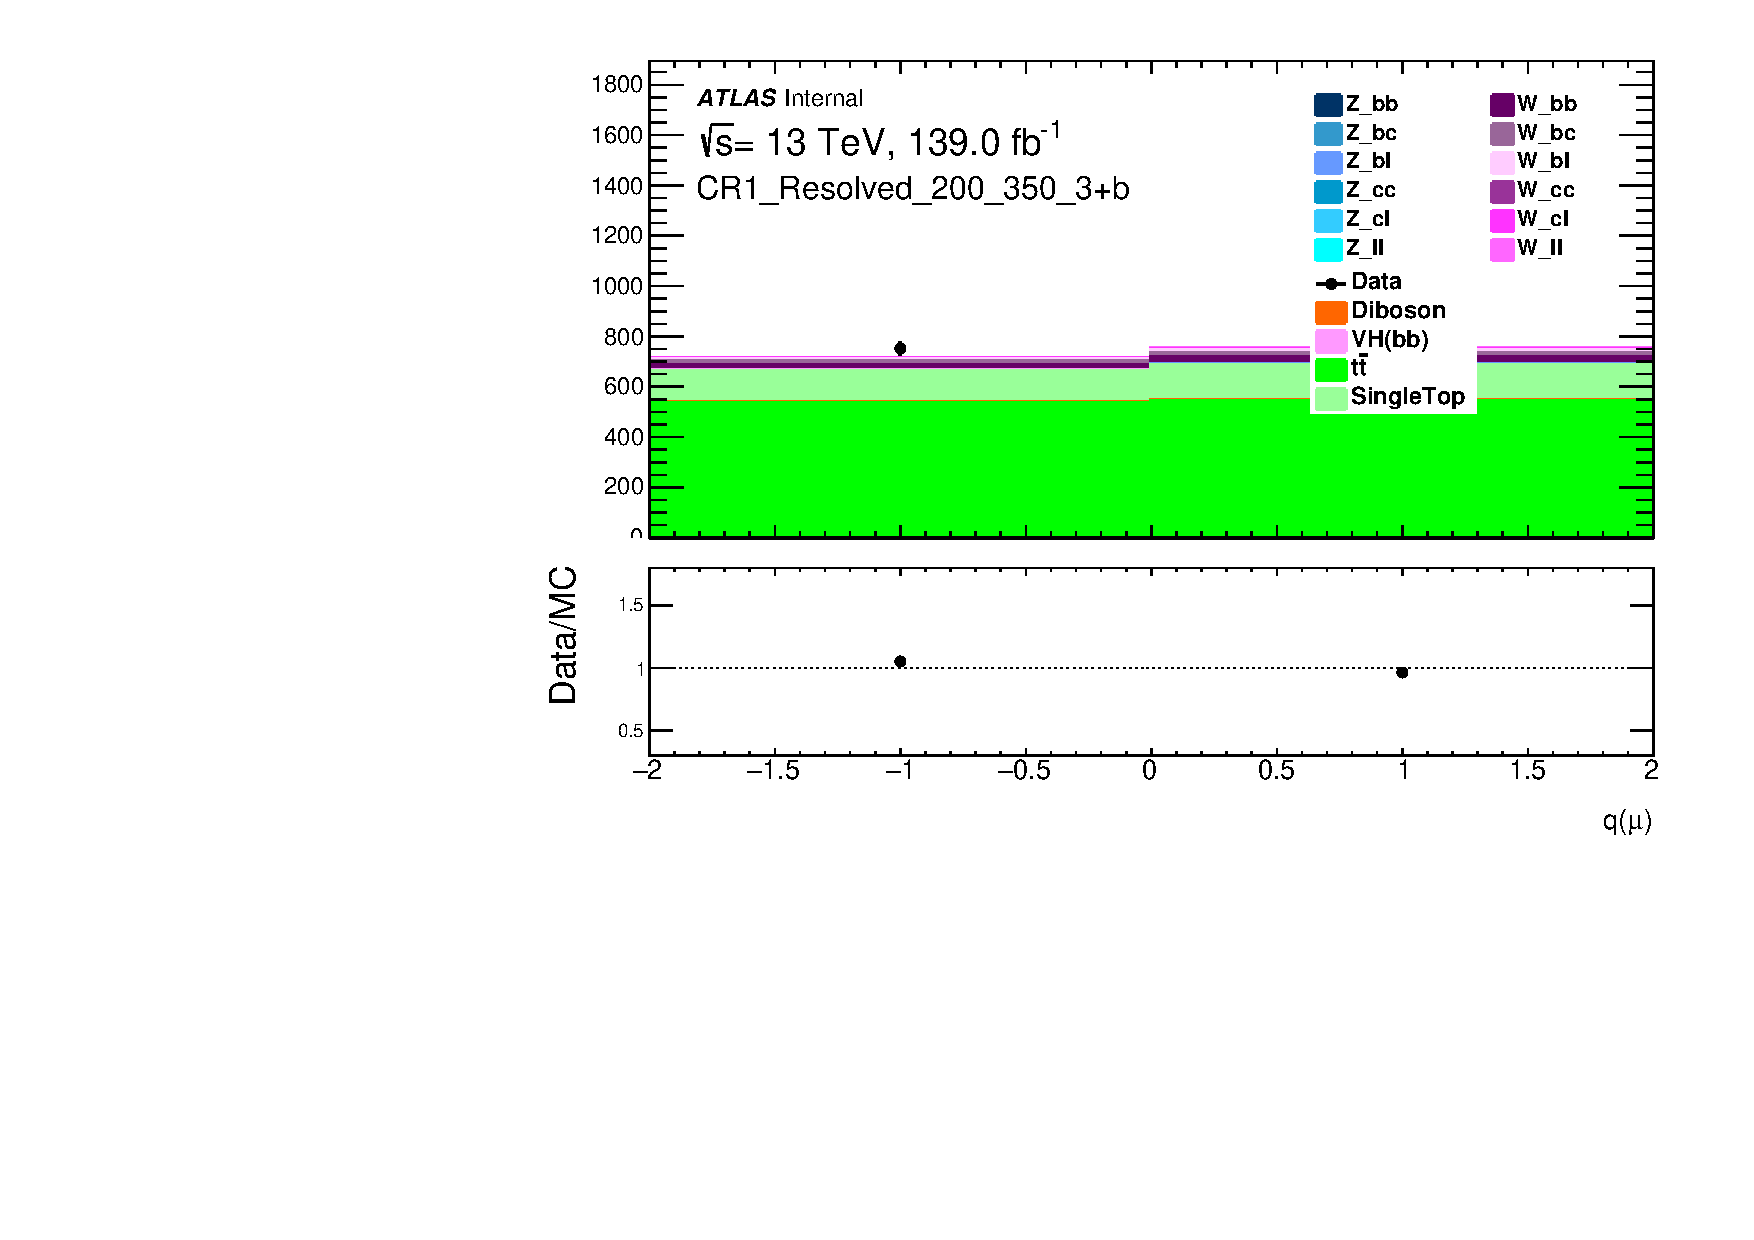
\includegraphics[width=0.46\linewidth]{chapters/c8/figures/1L/DataMC_MonoH_Nominal_CR1_Resolved_200_350_3+b_mu_charge.pdf}\\
    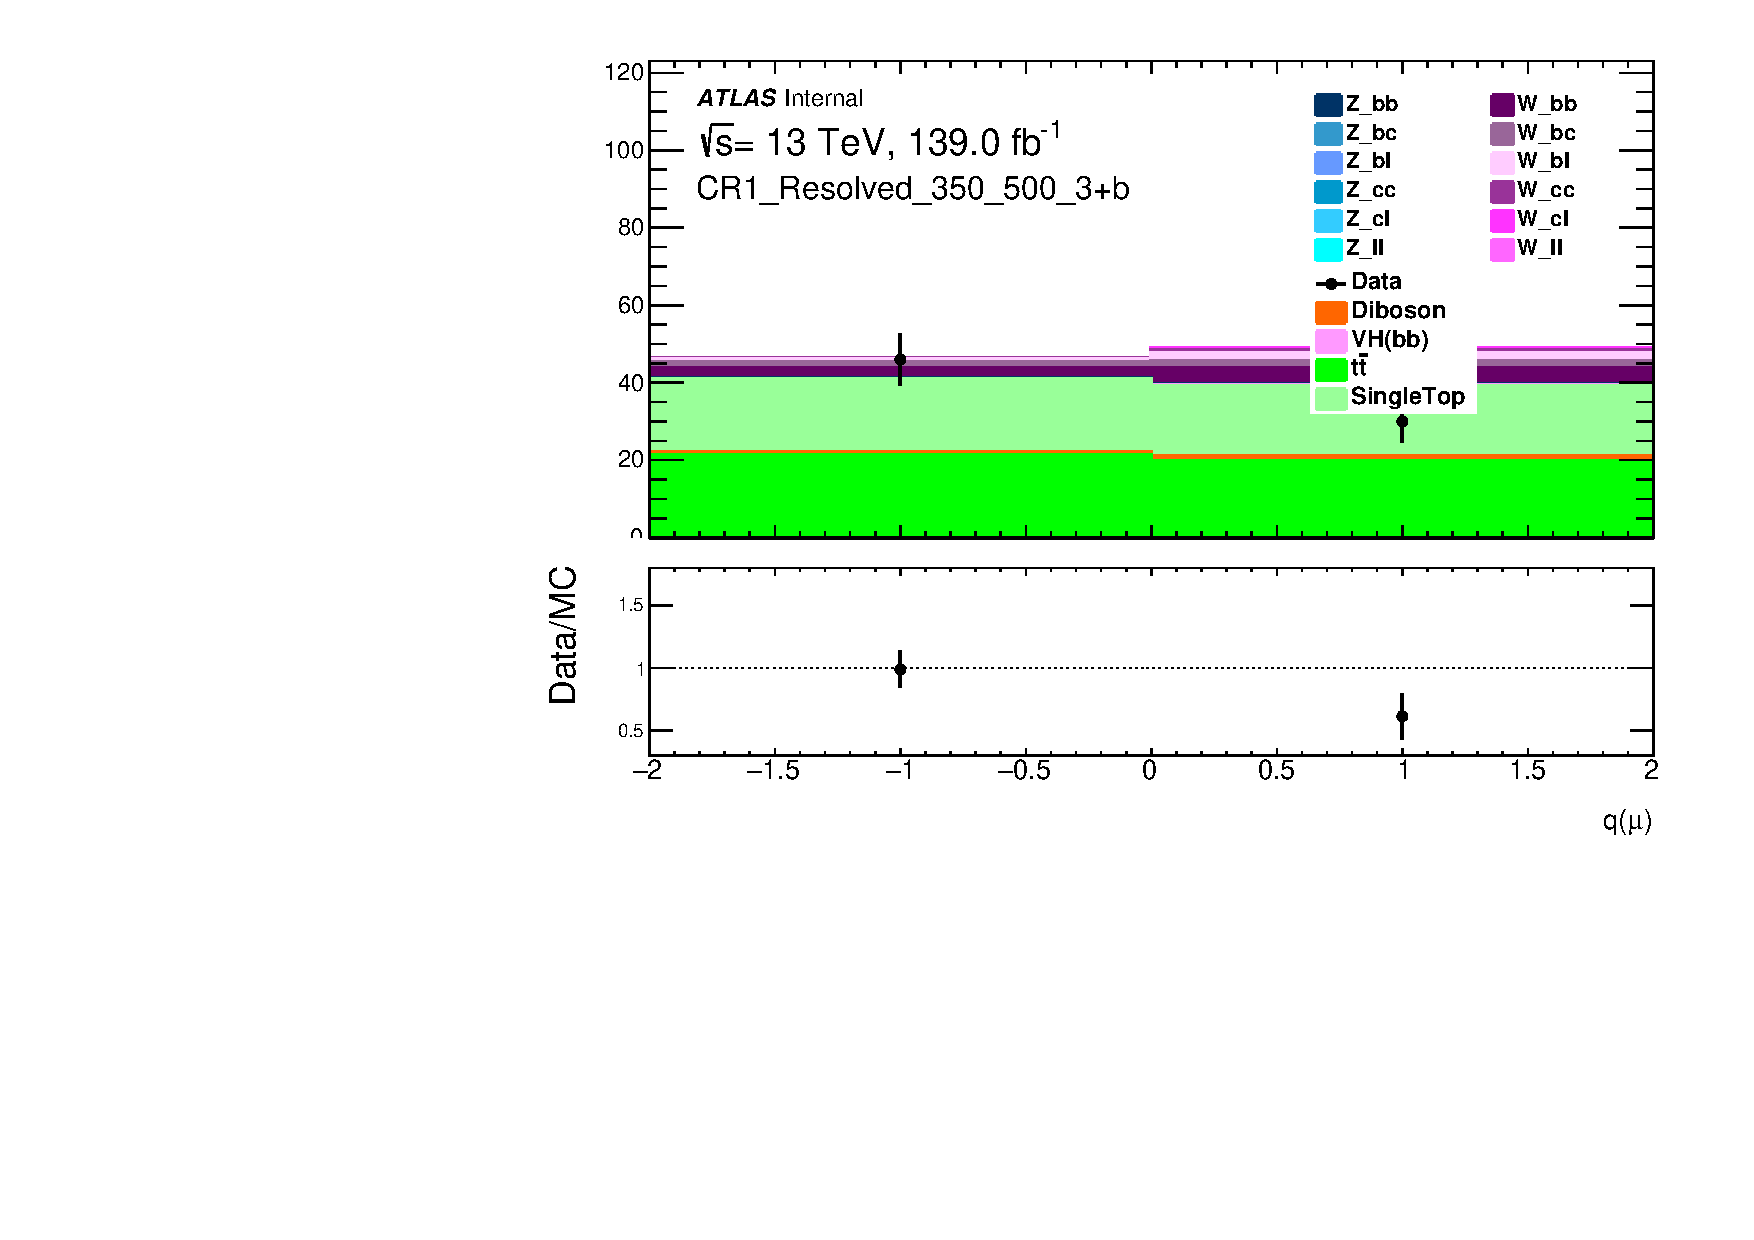
\includegraphics[width=0.46\linewidth]{chapters/c8/figures/1L/DataMC_MonoH_Nominal_CR1_Resolved_350_500_3+b_mu_charge.pdf}
    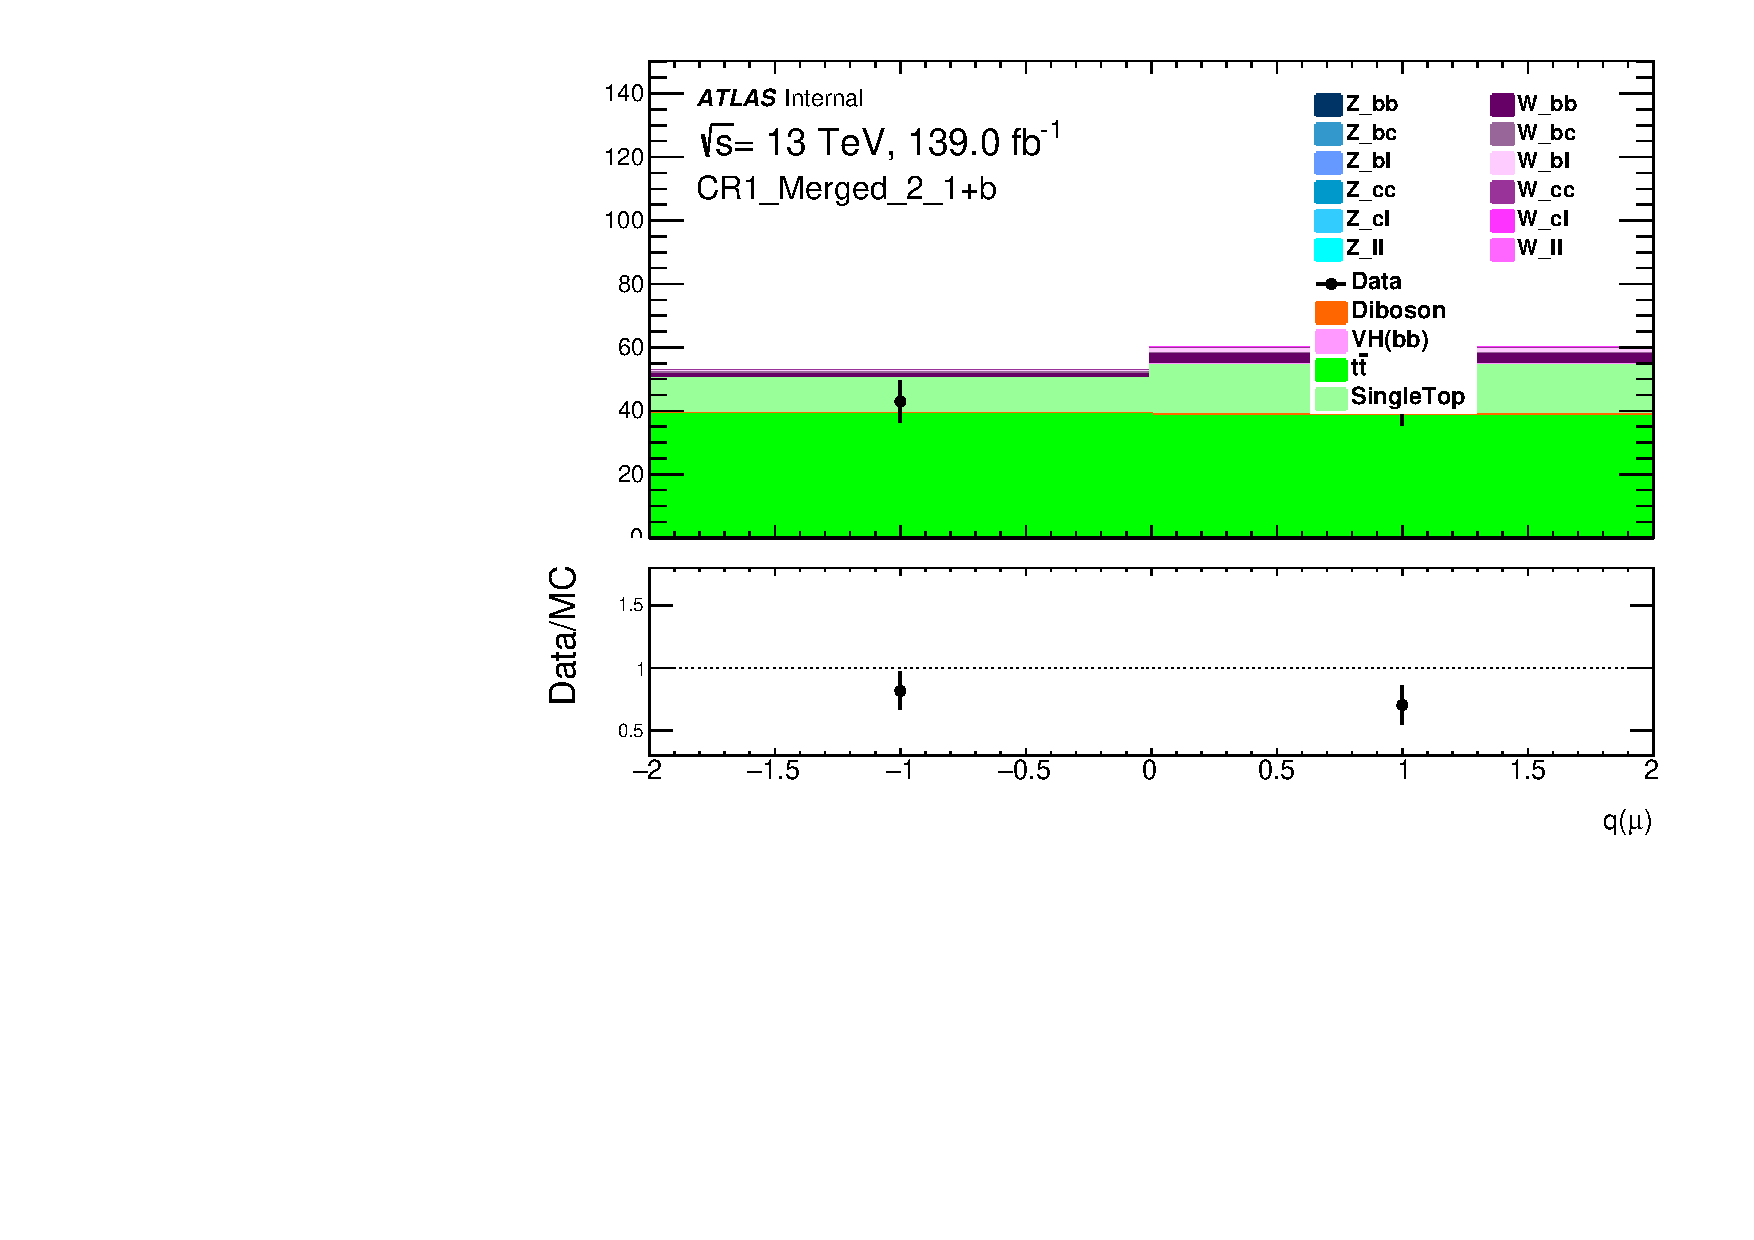
\includegraphics[width=0.46\linewidth]{chapters/c8/figures/1L/DataMC_MonoH_Nominal_CR1_Merged_2_1+b_mu_charge.pdf}
    \caption{Muon charge distribution in the different \met regions with least 3 $b$-tagged jets in the 1-lepton channel.}
    \label{fig:data-mc-1l-mu-charge-3+b}
\end{figure}

\begin{figure}[!htb]
    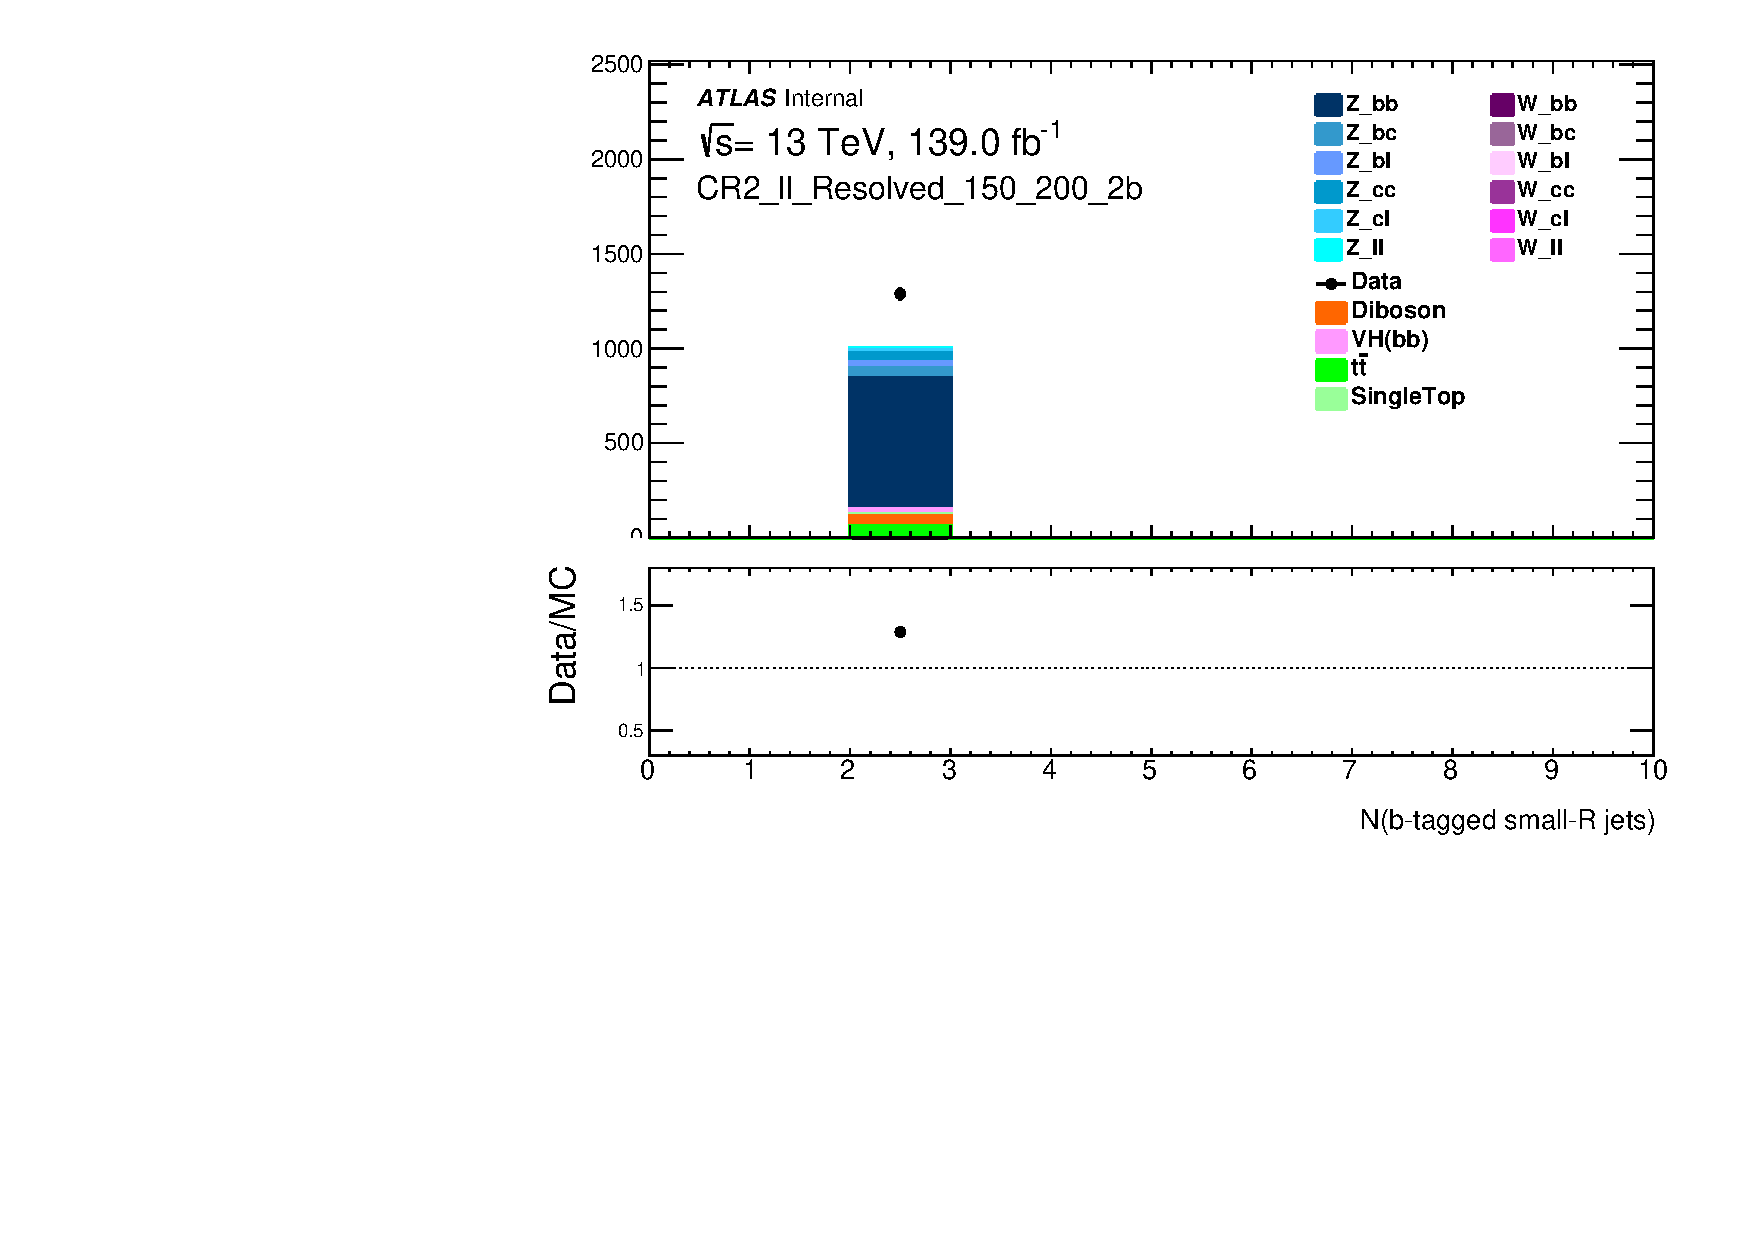
\includegraphics[width=0.46\linewidth]{chapters/c8/figures/2L/DataMC_MonoH_Nominal_CR2_ll_Resolved_150_200_2b_N_BJets_04.pdf}
    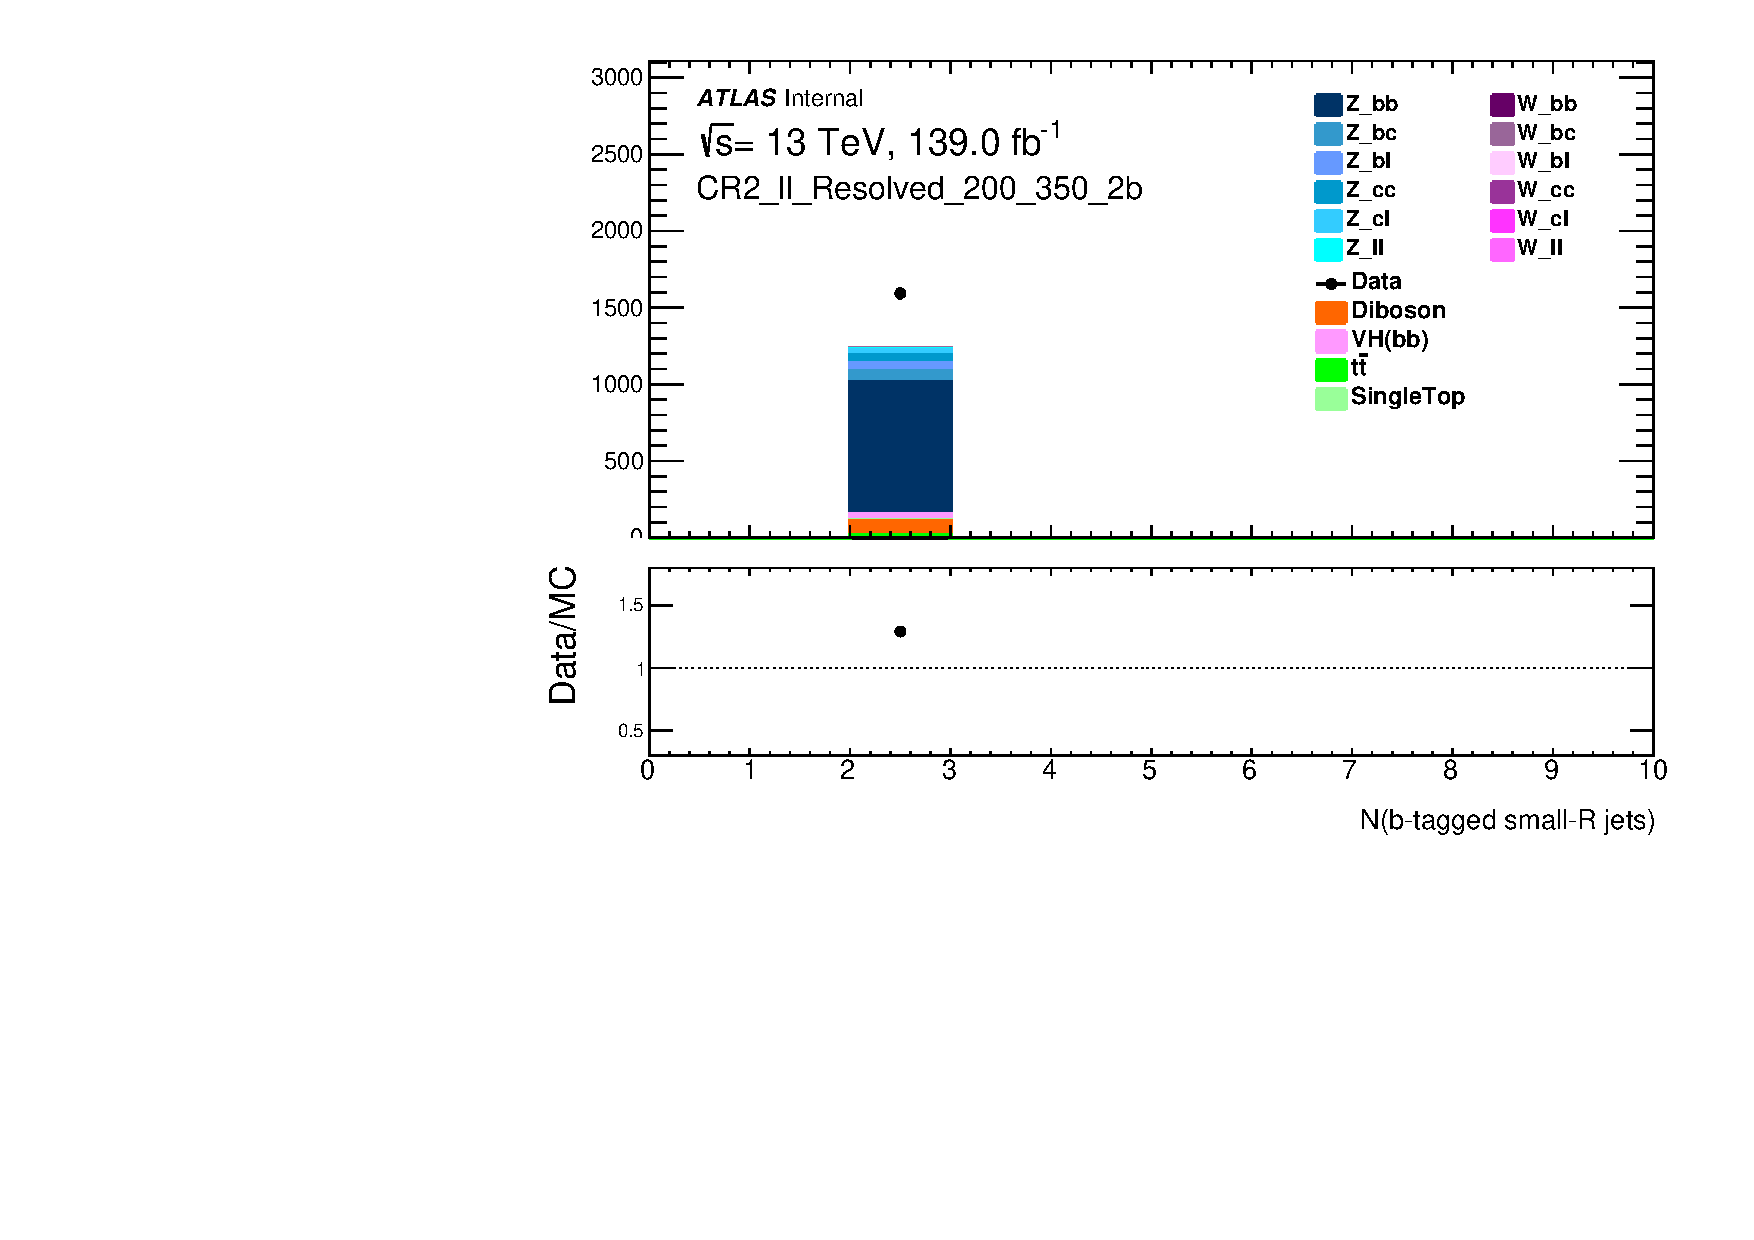
\includegraphics[width=0.46\linewidth]{chapters/c8/figures/2L/DataMC_MonoH_Nominal_CR2_ll_Resolved_200_350_2b_N_BJets_04.pdf}\\
    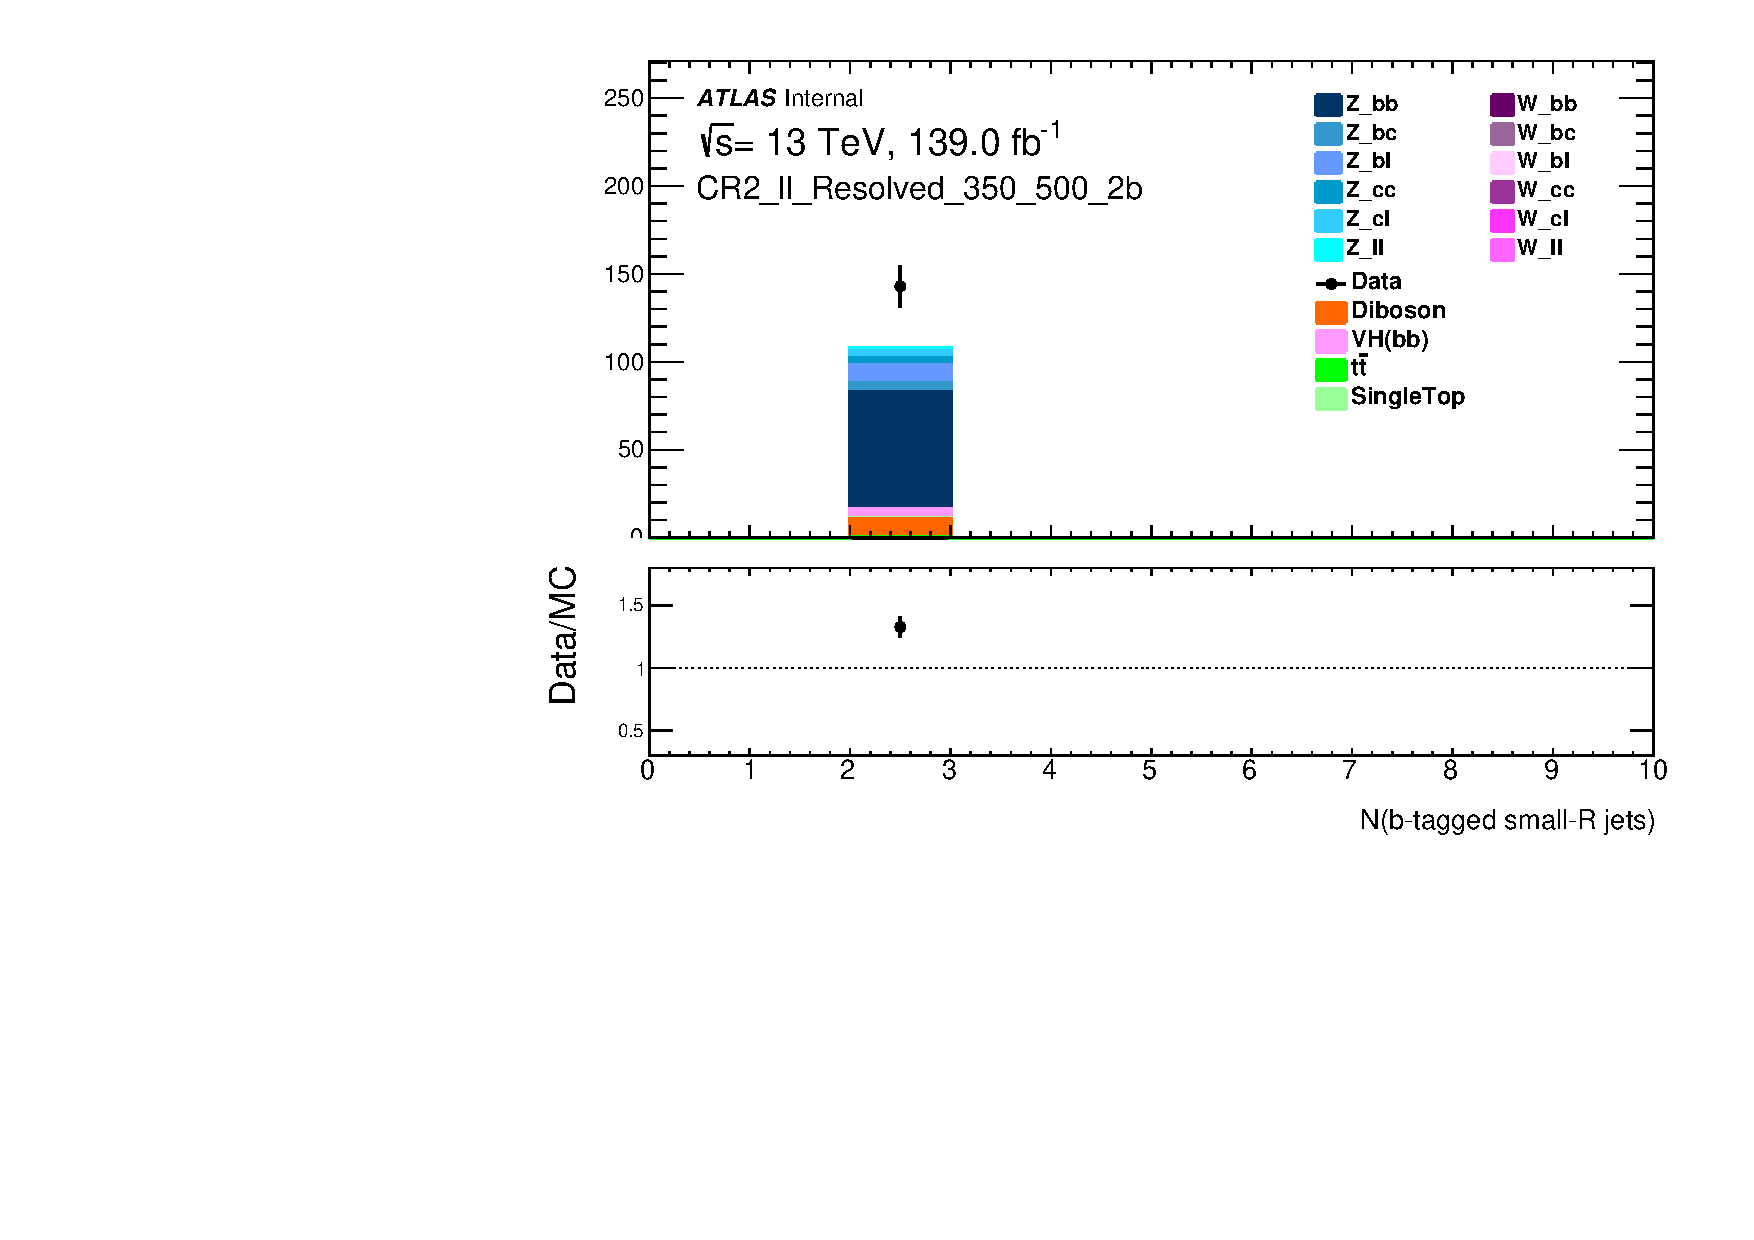
\includegraphics[width=0.46\linewidth]{chapters/c8/figures/2L/DataMC_MonoH_Nominal_CR2_ll_Resolved_350_500_2b_N_BJets_04.pdf}
    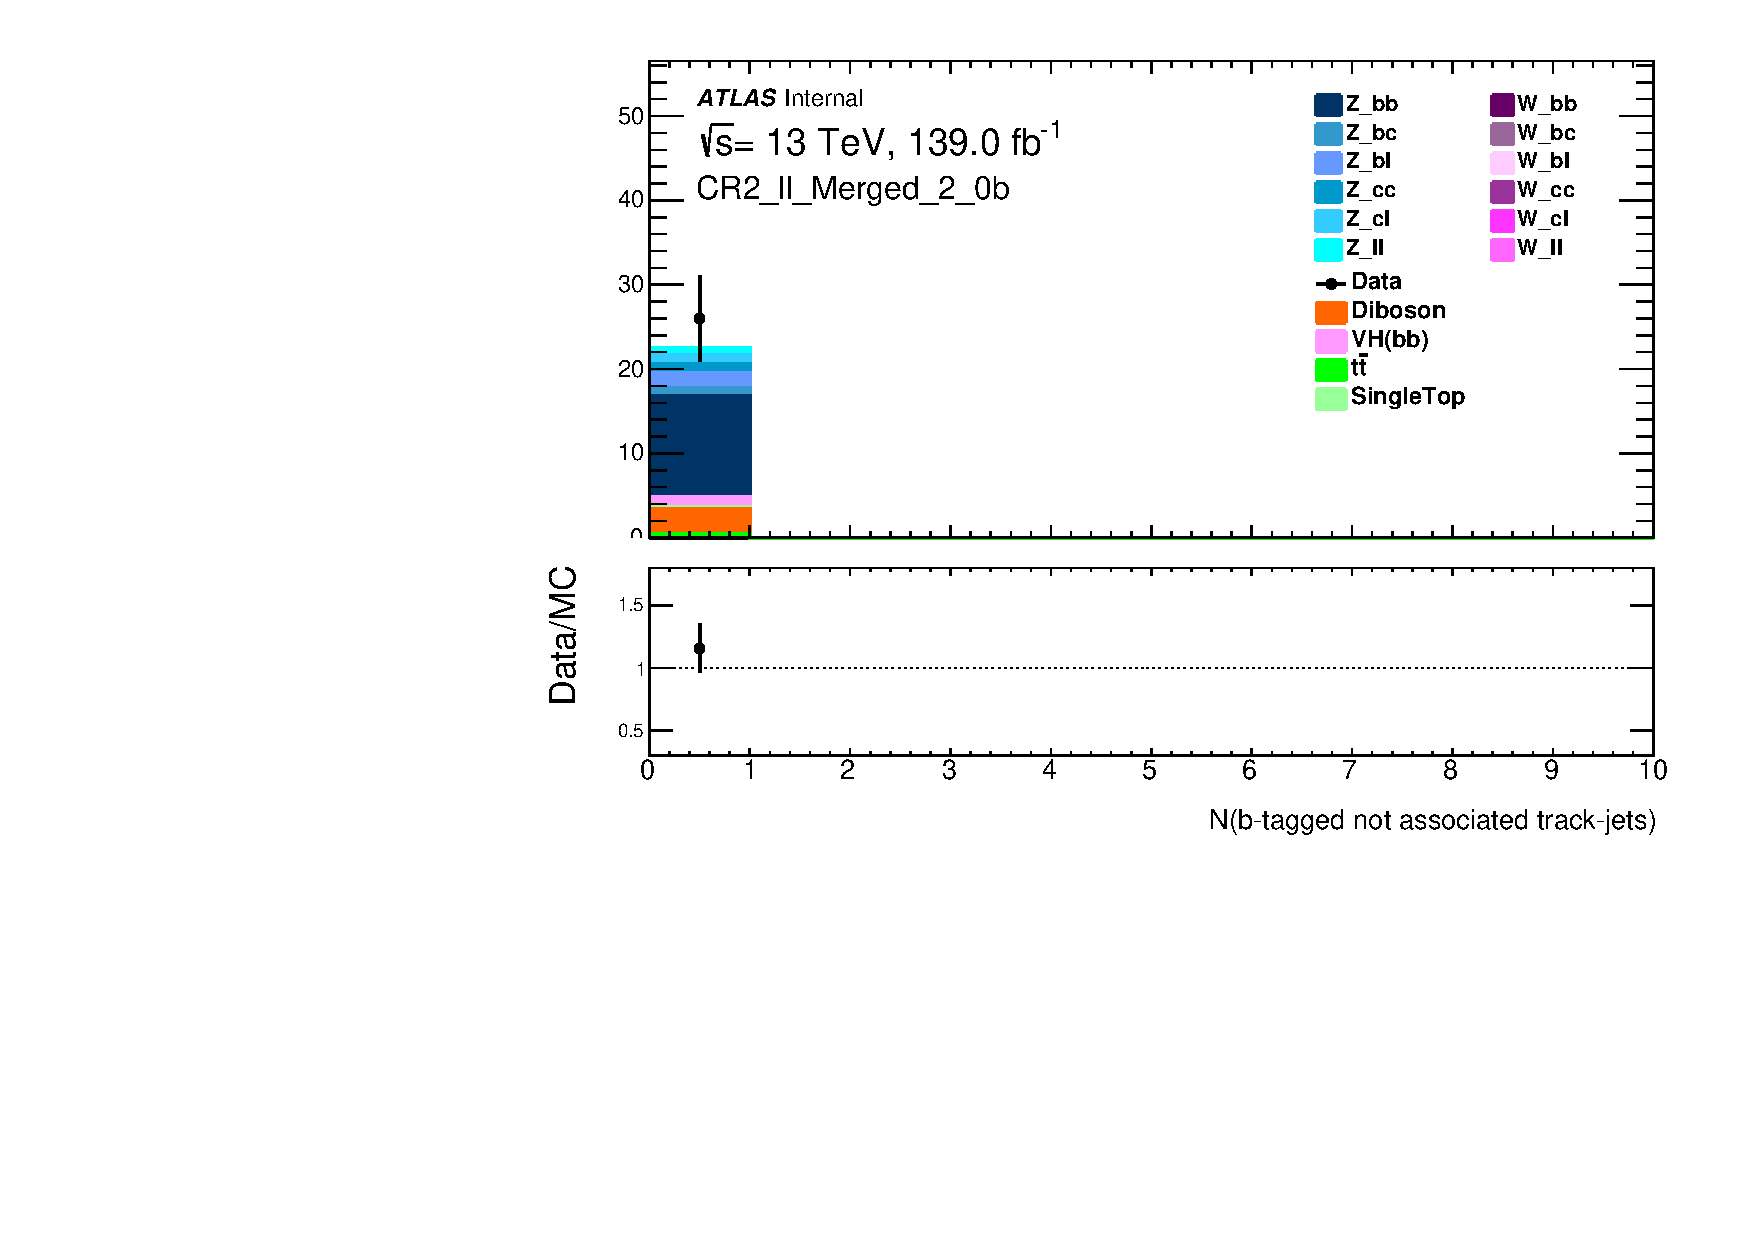
\includegraphics[width=0.46\linewidth]{chapters/c8/figures/2L/DataMC_MonoH_Nominal_CR2_ll_Merged_2_0b_N_BTags_not_associated_02.pdf}
    \caption{Total yields in the 2-lepton control region for different \met regions with 2 $b$-tagged jets.}
    \label{fig:data-mc-2l-ll-nb-2b}
\end{figure}
  
\begin{figure}[!htb]
    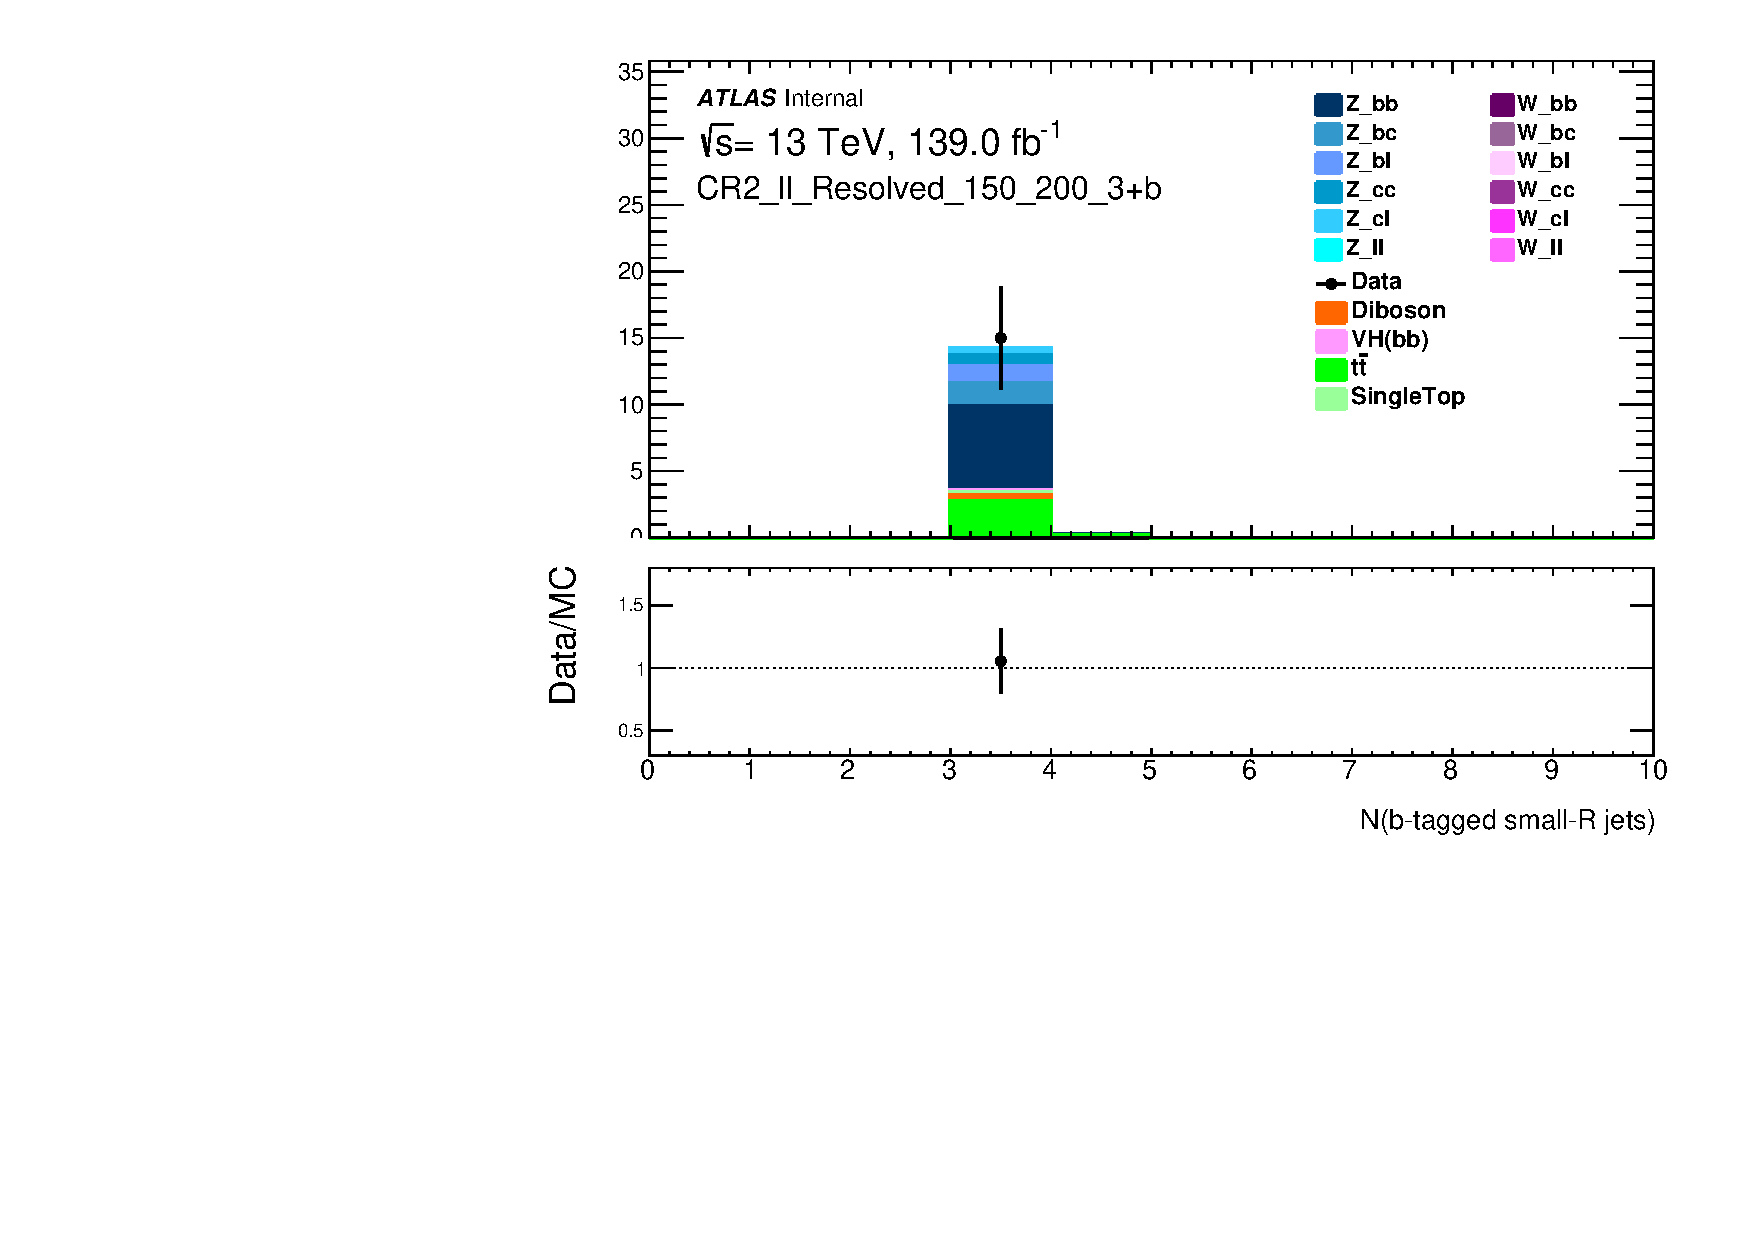
\includegraphics[width=0.46\linewidth]{chapters/c8/figures/2L/DataMC_MonoH_Nominal_CR2_ll_Resolved_150_200_3+b_N_BJets_04.pdf}
    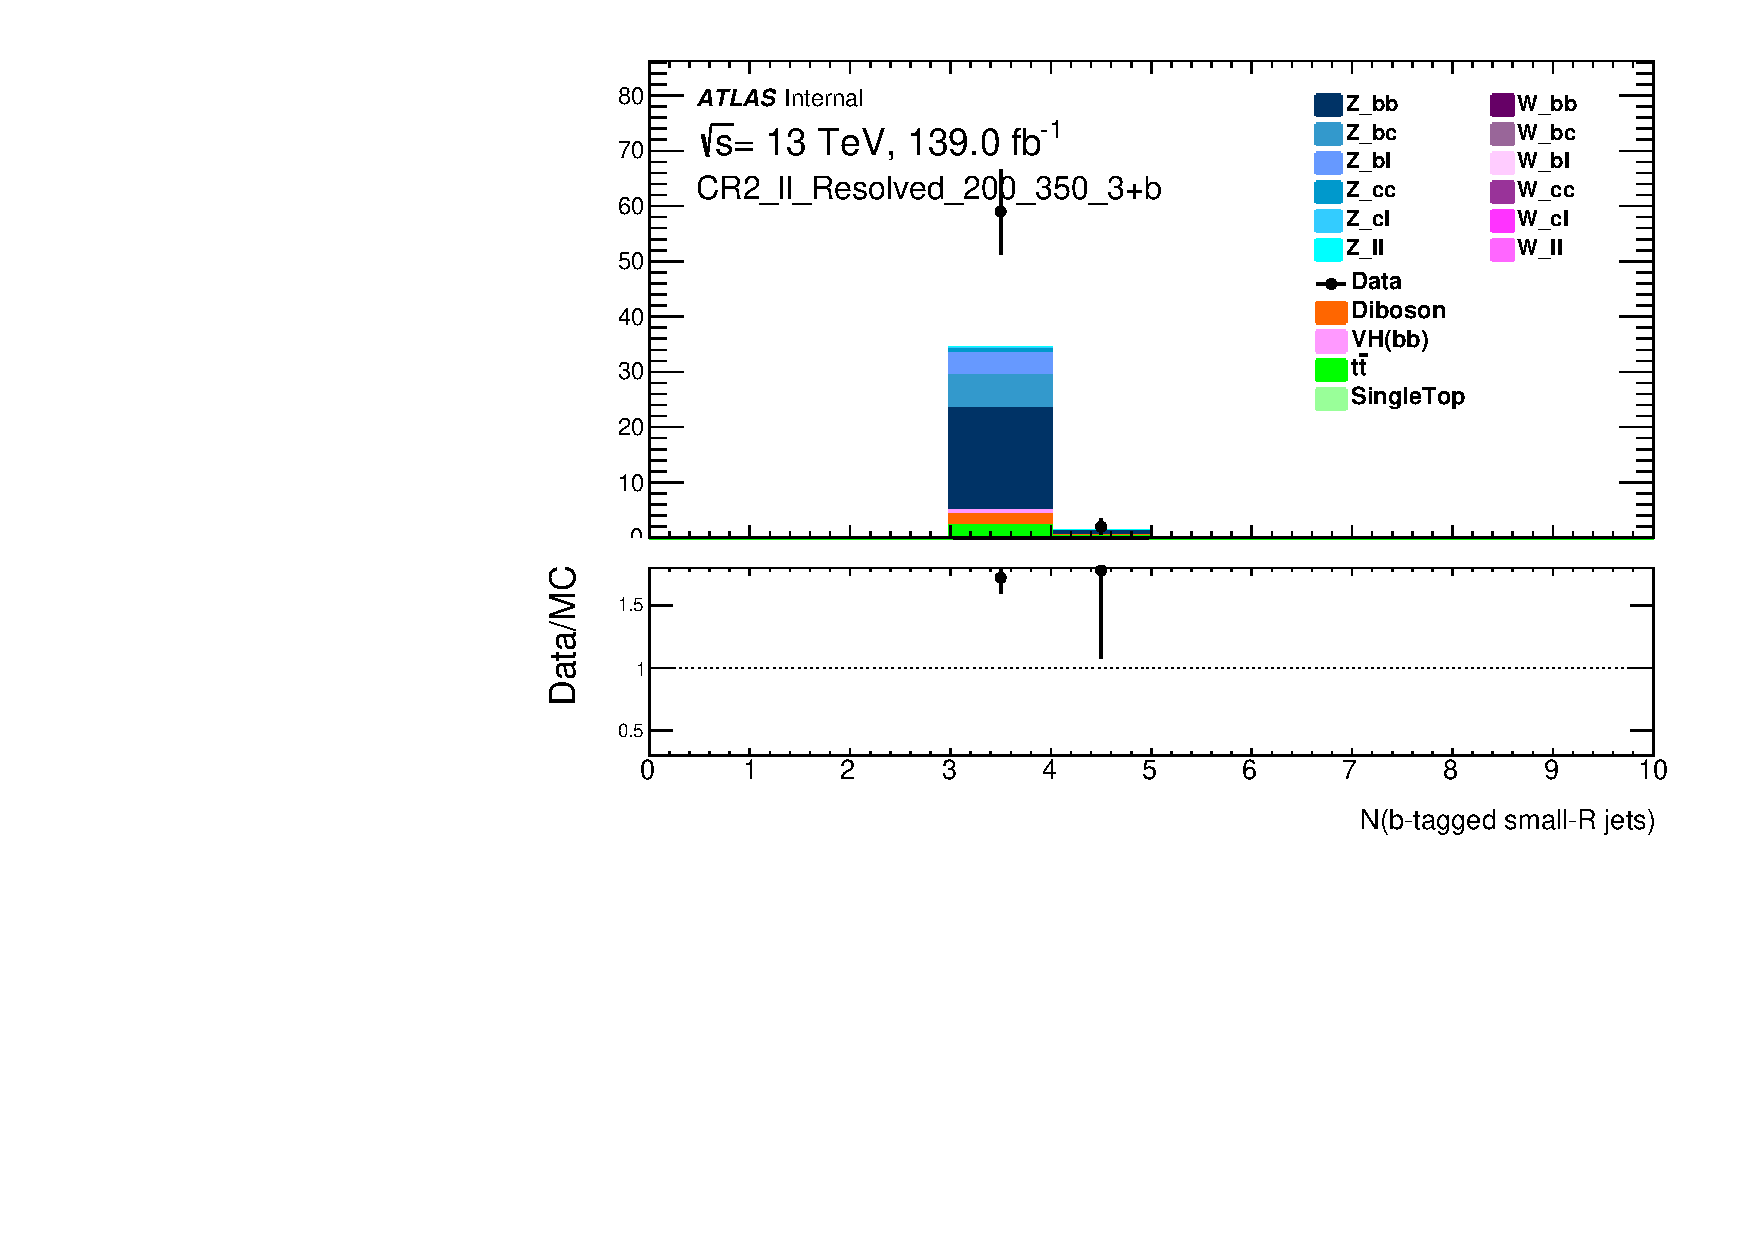
\includegraphics[width=0.46\linewidth]{chapters/c8/figures/2L/DataMC_MonoH_Nominal_CR2_ll_Resolved_200_350_3+b_N_BJets_04.pdf}\\
    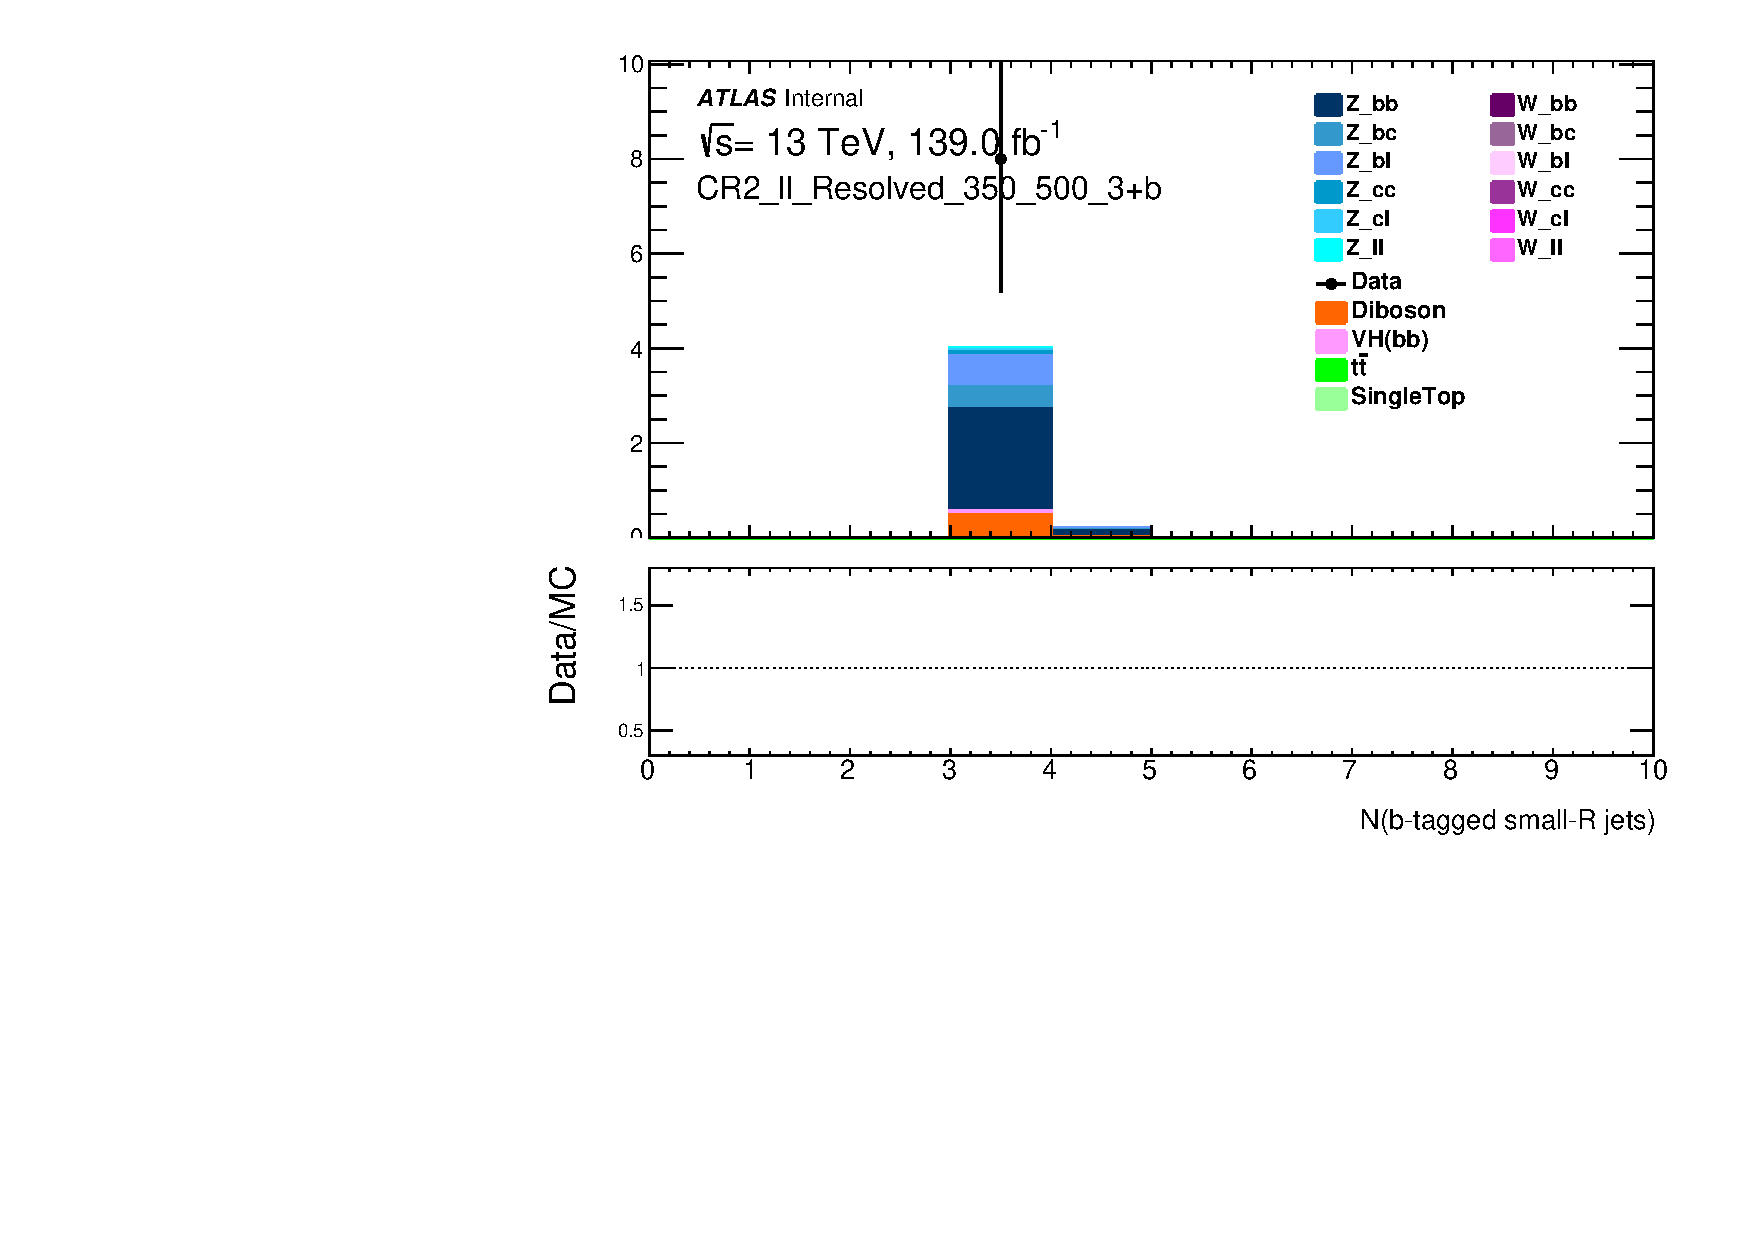
\includegraphics[width=0.46\linewidth]{chapters/c8/figures/2L/DataMC_MonoH_Nominal_CR2_ll_Resolved_350_500_3+b_N_BJets_04.pdf}
    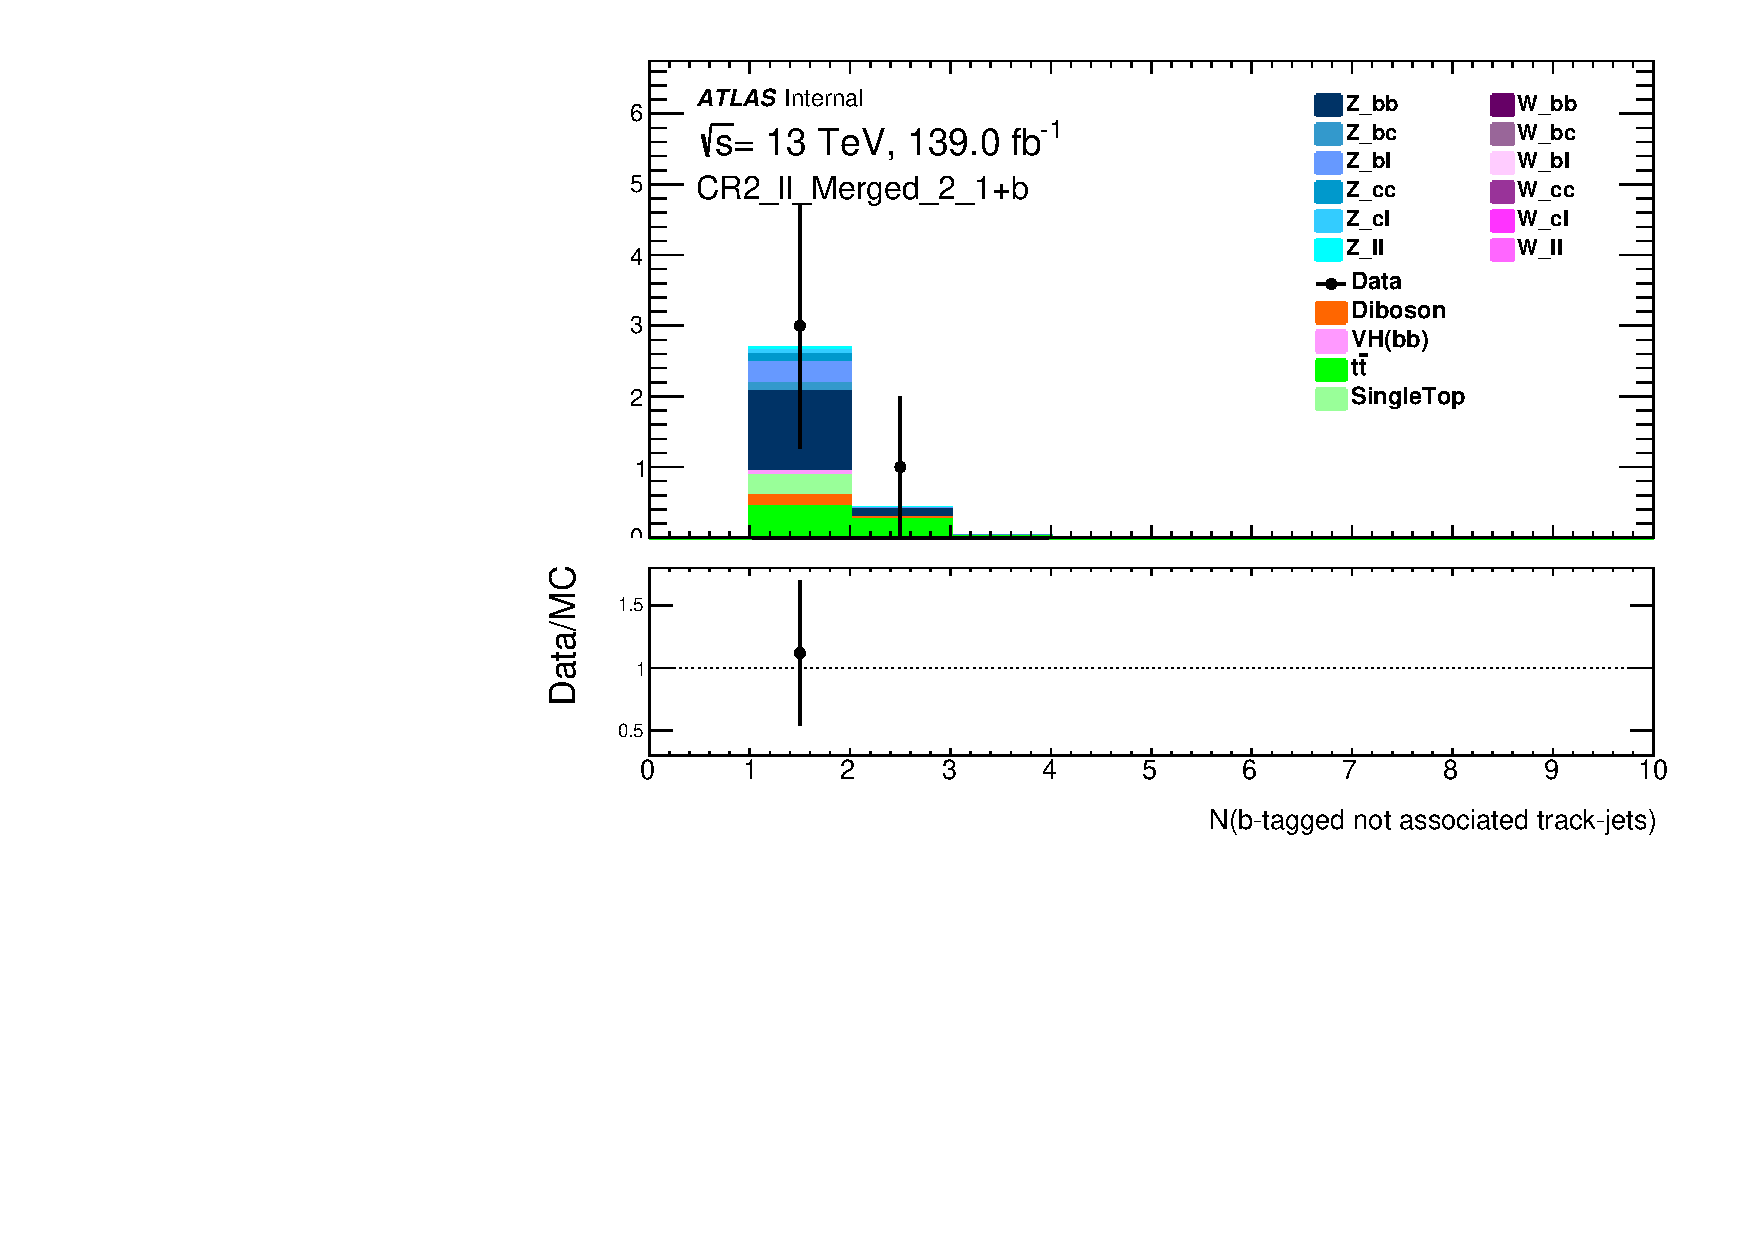
\includegraphics[width=0.46\linewidth]{chapters/c8/figures/2L/DataMC_MonoH_Nominal_CR2_ll_Merged_2_1+b_N_BTags_not_associated_02.pdf}
    \caption{Total yields in the 2-lepton control region for different \met regions with more than 2 $b$-tagged jets.}
    \label{fig:data-mc-2l-ll-nb-3+b}
\end{figure}
